% !TEX root = main.tex

\section{Analysis strategy}
\label{sec:strategy}

The selection of the signal, $B_s \to D_s K \pi \pi$, and calibration channel, $B_s \to D_s \pi \pi \pi$,
are outlined in Sect.~\ref{sec:Selection},
followed by the determination of the signal and background yields.
The  calibration channel is used to study the decay-time acceptance, see Sect.~\ref{sec:Acceptance},
and to calibrate the flavor tagging algorithms in Sect.~\ref{sec:Tagging}.
Moreover, the $B_s$ mixing frequency is measured in Sect.~\ref{ssec:timeNormFit}.
Afterwards, the CKM angle $\gamma$ is extracted from $B_s \to D_s K \pi \pi$ data using two different approaches:
the results of the phase-space integrated fit are presented in Sect.~\ref{ssec:timeFit},
while Sect.~\ref{sec:fullFit} discusses the significantly more complicated full time-dependent amplitude fit.
The systematic uncertainties of both methods are determined in Sect.~\ref{sec:Systematics},
before we compare the results and conclude in Sect.~\ref{sec:Summary}.


%\clearpage
\section{Data samples and event selection}
\label{sec:Selection}

\subsection{Stripping and Trigger selection}

The dataset used for this analysis corresponds to $1 \invfb$ of proton-proton collision data
collected in 2011 with a centre of mass energy $\sqrt{s} = 7\tev$,  $2 \invfb$  collected in
2012 with $\sqrt{s} = 7\tev$ and $4 \invfb$  collected in
2015/2016/2017 with $\sqrt{s} = 13\tev$.
Candidate $\Bs\to\Ds\kaon\pion\pion$ ($\Bs\to\Ds\pion\pion\pion$) decays are reconstructed using the
\textsf{B02DKPiPiD2HHHPIDBeauty2CharmLine} (\textsf{B02DPiPiPiD2HHHPIDBeauty2CharmLine})
line of the \textsf{BHadronCompleteEvent} stream of  
\textsf{Stripping21r1} (2011), \textsf{Stripping21} (2012),
\textsf{Stripping24r1} (2015)  and \textsf{Stripping28r1p1} (2016)
and \textsf{Stripping29r2} (2017).
Both stripping lines employ the same selection cuts, listed in Appendix \ref{sec:StripAndTrigger}, except for the PID requirement on the bachelor kaon/pion.

Events that pass the stripping selection are further required to fulfill the following trigger requirements:
at the hardware stage, the $\Bs$ candidates are required to be TOS on the \textsf{L0Hadron} trigger or TIS on \textsf{L0Global};
at Hlt1, $\Bs$ candidates are required to be TOS on the \textsf{Hlt1TrackAllL0} (\textsf{Hlt1TrackMVA} or \textsf{Hlt1TwoTrackMVA}) trigger line for Run-I (Run-II) data;
at Hlt2, candidates have to be TOS on either one of the 2, 3 or 4-body topological trigger lines or the inclusive $\phi$ trigger. 
More details on the used HLT lines are given in Appendix \ref{sec:StripAndTrigger}.

Due to a residual kinematic dependence on whether the event is triggered by \textsf{L0Hadron} or not and on the data taking condition,
the analysis is performed in four disjoint categories: 
$[\text{Run-I,}\textsf{L0-TOS}]$, $[\text{Run-I,}\textsf{L0-TIS}]$, $ [\text{Run-II,}\textsf{L0-TOS}]$ and $ [\text{Run-II,}\textsf{L0-TIS}]$,
where for simplicity we denote  $\textsf{L0Hadron-TOS}$ as $\textsf{L0-TOS}$ and $ (\textsf{L0Global-TIS} \text{ and not } \textsf{L0Hadron-TOS})$ as $\textsf{L0-TIS}$.
 


\subsection{Offline selection}

The offline selection, in particular the requirements on the $D_s$ hadron, are guided by the previous analyses of 
$B_s \to D_s K/\pi$, $B_d \to D^0 \pi$ as well as the branching fraction measurement of $\Bs\to\Ds\kaon\pion\pion$ decays.
Tables \ref{table:selDs} and \ref{table:selBs} summarize all selection requirements which are described in the following.
Throughout the note, we abbreviate $\Bs\to\Ds X_{s}(\to\kaon\pion\pion)$ and $\Bs\to\Ds X_{d}(\to\pion\pion\pion)$.
%identifying $X_{s}\to\kaon\pion\pion$ and $X_{d}\to\pion\pion\pion$ as the various resonances through which the decays proceed. 
%A two-fold approach is used to isolate the signal candidates from data passing the stripping line. 
%First, loose cuts are applied to suppress the combinatorial background, 
%Following this, a multivariate classifier is trained which combines the information of several input variables, including their correlation, into one powerful discriminator
%between signal and combinatorial background. 

Given the high number of $pp$ interactions per bunch crossing, a large fraction
of events have more than one reconstructed PV. 
We choose the 'best' PV to be the one to which the 
$B_s$ candidate has the smallest $\chi^2_{IP}$.
In instances where the association of the $B_s$ candidate to the best PV is wrong,
the decay time of this candidate will be incorrect. 
These wrongly associated candidates
are rejected by requiring that the $B_s$ $\chi^2_{IP}$ with respect to any other PV is sufficiently higher than with respect to the best PV 
($\Delta \chi^2_{IP} = \chi^2_{\text{IP,SECONDBEST}} - \chi^2_{\text{IP,BEST}} > 20$ ).
Events with only a single PV are not affected.

In order to clean up the sample and to align the Run-I to the slightly tighter Run-II stripping selection, we apply the following loose cuts to the b-hadron:
\begin{itemize}
\item DIRA $>$ 0.99994
\item min IP $\chi^{2}$ $<$ 16 to the best PV,
\item FD $\chi^{2}$ $>$ 100 to the best PV,
\item Vertex $\chi^{2}$/nDoF $<$ 8.
%\item ($Z_{\Ds}-Z_{\Bs}$) $>$ 0 , where $Z_{M}$ is the z-component of the position $\vec{x}$ of the decay vertex for the $\Bs$/$\Ds$ meson.
\end{itemize}    
The cut on the $B_s$ decay-time is tightened with respect to the stripping selection ($t > 0.2 \ps$) because, while offline we use the decay-time determined for a DTF in which the PV position, the $D_s$ and the $B_s$ mass are constrained, in the stripping the simple decay-time returned by a kinematic fit is used. 
The difference between these two decay-times extends up to 0.1 ps, thus cutting at 0.4 ps avoids any boundary effects and simplifies the time-acceptance studies.
We further remove outliers with poorly estimated decay times ($\delta t< 0.15 \ps$).

We reconstruct the $\Bs\to\Ds h\pion\pion$ decay through three different final states of the $\Ds$ meson: $\Ds\to\kaon\kaon\pion$, $\Ds\to\pion\pion\pion$ and $\Ds\to\kaon\pion\pion$.
Of those, $\Ds\to\kaon\kaon\pion$ is the most prominent one,
while $\mathcal{BR}(\Ds\to\pion\pion\pion) \approx 0.2\cdot\mathcal{BR}(\Ds\to\kaon\kaon\pion)$ and $\mathcal{BR}(\Ds\to\kaon\pion\pion) \approx 0.12\cdot\mathcal{BR}(\Ds\to\kaon\kaon\pion)$ holds for the others. 
For the $\kaon\kaon\pion$  final state we make use of the well known resonance structure;
the decay proceeds either via the narrow $\phiz$ resonance, the broader $\Kstarz$ resonance or (predominantly) non-resonant.
Within the $\phiz$ resonance region the sample is already sufficiently clean after the stripping so that we do not impose additional criteria on the $D_s$ daughters.
For the $\Kstarz$ and non-resonant regions consecutively tighter requirements on the particle identification and the $D_s$ flight-distance are applied. 
We apply global requirements (\ie independent of the $D_s$ Dalitz-plot position) for the other final states. All cuts are summarized in Table \ref{table:selDs}.


%Depending on the decay process being resonant or not, we apply additional PID requirements on this final state:
%
%\begin{itemize}
%\item resonant case: 
%\begin{itemize}
%\item $\Dsp\to\phiz\pip$, with $|M(\Kp\Km) - m_{\phiz}|$ $<$ 20 $\mevcc$ : no additional requirements, since $\phiz$ is narrow and almost pure $\Kp\Km$. 
%\item $\Dsp\to\Kstarzb\Kp$, with  $|M(\Km\pip) -m_{\Kstarz}|$ $<$ 75 $\mevcc$ :  $\dllkpi$ $>$ 0 for kaons, since this resonance is more than ten times broader than $\phiz$. 
%\end{itemize}
%\item non resonant case: $\dllkpi$ $>$ 5 for kaons, since the non resonant category has significant charmless contributions.
%\end{itemize}
%
%\begin{itemize}
%\item $\dllkpi$ $<$ 10 for all pions.
%\item $\dllppi$ $<$ 10 for all pions.
%\end{itemize}
 
 \subsubsection{Phase space region}
 \label{ssec:phasespace}

Due to the comparably low masses of the final state particles  with respect to the $B_s$ mass,
there is, in contrast to for example b-hadron to charmonia or charm decays, a huge phase-space available for the $\Bs\to\Ds\kaon\pion\pion$ decay.
For the invariant mass of the $K\pi\pi$ subsystem it extends up to $3.4 \gev$.
It has however been observed that the decay proceeds predominantly through the low lying axial vector states $K_{1}(1270)$ and $K_{1}(1400)$, while
the combinatorial background is concentrated at high $K\pi\pi$ invariant masses ($m(K\pi\pi) > 2000 \mev$).
Moreover, the strange hadron spectrum above $2\gev$ is poorly understood experimentally such that a reliable extraction of the strong phase motion in that region is not possible.
We consequently choose to limit the considered phase space region to $m(K\pi\pi) < 1950 \mev$, which is right below the charm-strange threshold ($\Bs\to\Dsp\Dsm$).
 
 \clearpage
\subsubsection{Physics background vetoes}
 \label{ssec:vetoes}

We veto various physical backgrounds, which have either the same final state as our signal decay, or can contribute via a single misidentification of $\kaon \leftrightarrow \pion$, $\kaon\leftrightarrow\proton$ or $\pi \leftrightarrow\proton$. 
Depending on the $D_s$ final state different vetoes are applied in order to account for peaking backgrounds originating from charm meson or charmed baryon decays.
\begin{enumerate}

\item $\Ds^-\to\kaon^+\kaon^-\pion^-$

\begin{enumerate}
	\item $\Dm \to\Kp\pim\pim$: \\
	Possible with $\pim\rightarrow\Km$ misidentification, vetoed by requiring 
	$m(\Kp K^-_\pi \pim) \ne m(D^-) \pm 40$ MeV 
	or the $\Km$ has to fulfill more stringent PID criteria depending on the resonant region (see Table  \ref{table:selDs}).
	
	\item $\Lambda_c^- \to \Kp \bar p \pim $:  \\
	Possible with $\bar p \rightarrow\Km$ misidentification, vetoed by requiring
	$m(\Kp K^-_p \pim) \ne m(\Lambda_c) \pm 40$ MeV
	or the $\Km$ has to fulfill more stringent PID criteria depending on the resonant region (see Table  \ref{table:selDs}).
	
	\item $\Dz\to\kaon\kaon$: \\
	$\Dz$ combined with a random $\pion$ can fake a $\Ds\to\kaon\kaon\pion$ decay, 
	vetoed by requiring $m(\kaon\kaon) <  1840 \mev$. 
\end{enumerate}

\item $\Ds^-\to\pion^+\pion^-\pion^-$

\begin{enumerate}
%        \item $\Dm \to\Kp\pim\pim$: 
%	possible with single missID of $\Km\rightarrow\pim$: $m(\pip_K \pim \pim) is shifted to lower masses and 

%	\item $\Lambda_c^- \to \Kp \bar p \pim $: \\ 
%	Possible with double missID of $\bar p \rightarrow \pim$ and $\Kp \to \pip$

%	\item $\Lambda_c^- \to \pip \bar p \pim $: \\
%	Possible with single missID of $\bar p \rightarrow \pim$, vetoed by requiring
%	$m(\pip \pi^-_p \pim) \ne m(\Lambda_c) \pm 30$ MeV
%	or PIDp($\pim$) $< 0$ for each $\pim$.

	\item $\Dz\to\pion\pion$: \\
	$\Dz$ combined with a random $\pion$ can fake a $\Ds\to\pion\pion\pion$ decay, 
		vetoed by requiring both possible combinations to have $m(\pion\pion) < 1700 \mev$.
%	Same final state, vetoed by requiring $\left( M(\pi\pi\pim) - m(\pi\pi) \right) >  155 \mev$. 

\end{enumerate}

\item $\Ds^- \to K^- \pion^+\pion^-$

\begin{enumerate}

%	\item $\Dm \to\Kp\pim\pim$: \\
%	Possible with double missID of $\Kp \rightarrow\pip$ and $\pim \to \Km$

	\item $\Dm \to\pim\pip\pim$:  \\
	Possible with $\pim\rightarrow\Km$ misidentification, vetoed by requiring 
	$m(K^-_\pi \pip \pim) \ne m(D^-) \pm 40$ MeV 
	or PIDK($\Kp$) $> 15$.
	
%	\item $\Lambda_c^- \to \Kp \bar p \pim $: \\ Possible with double missID of $\bar p \rightarrow \Km$ and $\Kp \to \pip$
	
	\item $\Lambda_c^- \to \bar p \pip \pim $: \\
	Possible with $\bar p \rightarrow \Km$ misidentification, vetoed by requiring
	$m(K^-_p \pip \pim) \ne m(\Lambda_c) \pm 40$ MeV
	or PIDK($\Km$) $-$ PIDp($\Km$) $> 5$.
	
	\item $\Dz\to\kaon\pion$: \\
%	Same final state, vetoed by requiring $\left( M(K\pi\pim) - m(K\pi) \right) >  155 \mev$. 
	$\Dz$ combined with a random $\pion$ can fake a $\Ds\to\kaon\pion\pion$ decay, 
		vetoed by requiring both possible combinations to have $m(\kaon\pion) < 1750 \mev$.
\end{enumerate}

\end{enumerate}
The effects of these veto cuts are illustrated in Figs.~\ref{fig:vetoD},\ref{fig:vetoLambda} and \ref{fig:vetoD0}.
To reduce cross-feed from our calibration channel into the signal channel and vice-versa we require tight PID cuts on the ambiguous bachelor track; 
for the signal channel we apply $\text{PIDK}(K^+) >  10$ and for the calibration channel $\text{PIDK}(\pip) < 0$. 
In addition, we veto $\Bs\to\Dsm\Dsp$ decays which is illustrated in Fig.~\ref{fig:vetoDs}.
 \clearpage
\begin{enumerate}

	\item $X_s^+ \to \Kp \pip \pim$:
		\begin{enumerate}
			\item $\Bs\to\Ds\pion\pion\pion$: \\
			Possible with $\pip \to \Kp$ misidentification, suppressed with PIDK($\Kp$) $>10$.
			
			\item $\Bs\to\Dsm (\Dsp \to \Kp \pip \pim)$: \\ Outside of considered phase-space region, see Sec.~\ref{ssec:phasespace}.

			\item $\Bs\to\Dsm (\Dsp \to \Kp \Km \pip)$: \\
			To suppress $\Bs\to\Dsm \Kp \Km \pip$ background, possible with $\Km \to \pim$ misidentification, we require PIDK($\pim$) $< 0$.
			In case the invariant mass of the $\Kp \pip \pi$ system recomputed applying the kaon mass hypothesis to the pion
			is close to the $D_s$ mass ($m(\Kp \pip \pi^-_K) = m(D_s) \pm 20$ MeV),
			we further tighten the cut to PIDK($\pim$) $< -5$.
			%\item $\Bs \to \Dsm \mu \nu X$

		\end{enumerate}

	\item $X_d^+ \to \pip \pip \pim$:
		\begin{enumerate}
			\item $\Bs\to\Ds\kaon\pion\pion$: \\
			Possible with single missID of $\Kp \to \pip$, suppressed with PIDK($\pip$) $<0$.

			\item $\Bs\to\Dsm (\Dsp \to \pip \pip \pim)$:  \\ Outside of considered phase-space region, see Sec.~\ref{ssec:phasespace}.
			
			\item $\Bs\to\Dsm (\Dsp \to \Kp \pim \pip)$: \\
			Possible with single missID of $\Kp \to \pip$, vetoed by requiring
			$m(\pip \pi^+_K \pim) \ne m(D_s) \pm 20$ MeV or PIDK($\pip$) $<-5$ for both $\pip$.
			
			%\item $\Bs \to \Dsm \mu \nu X$

		\end{enumerate}
\end{enumerate}


\begin{figure}[h]
\centering
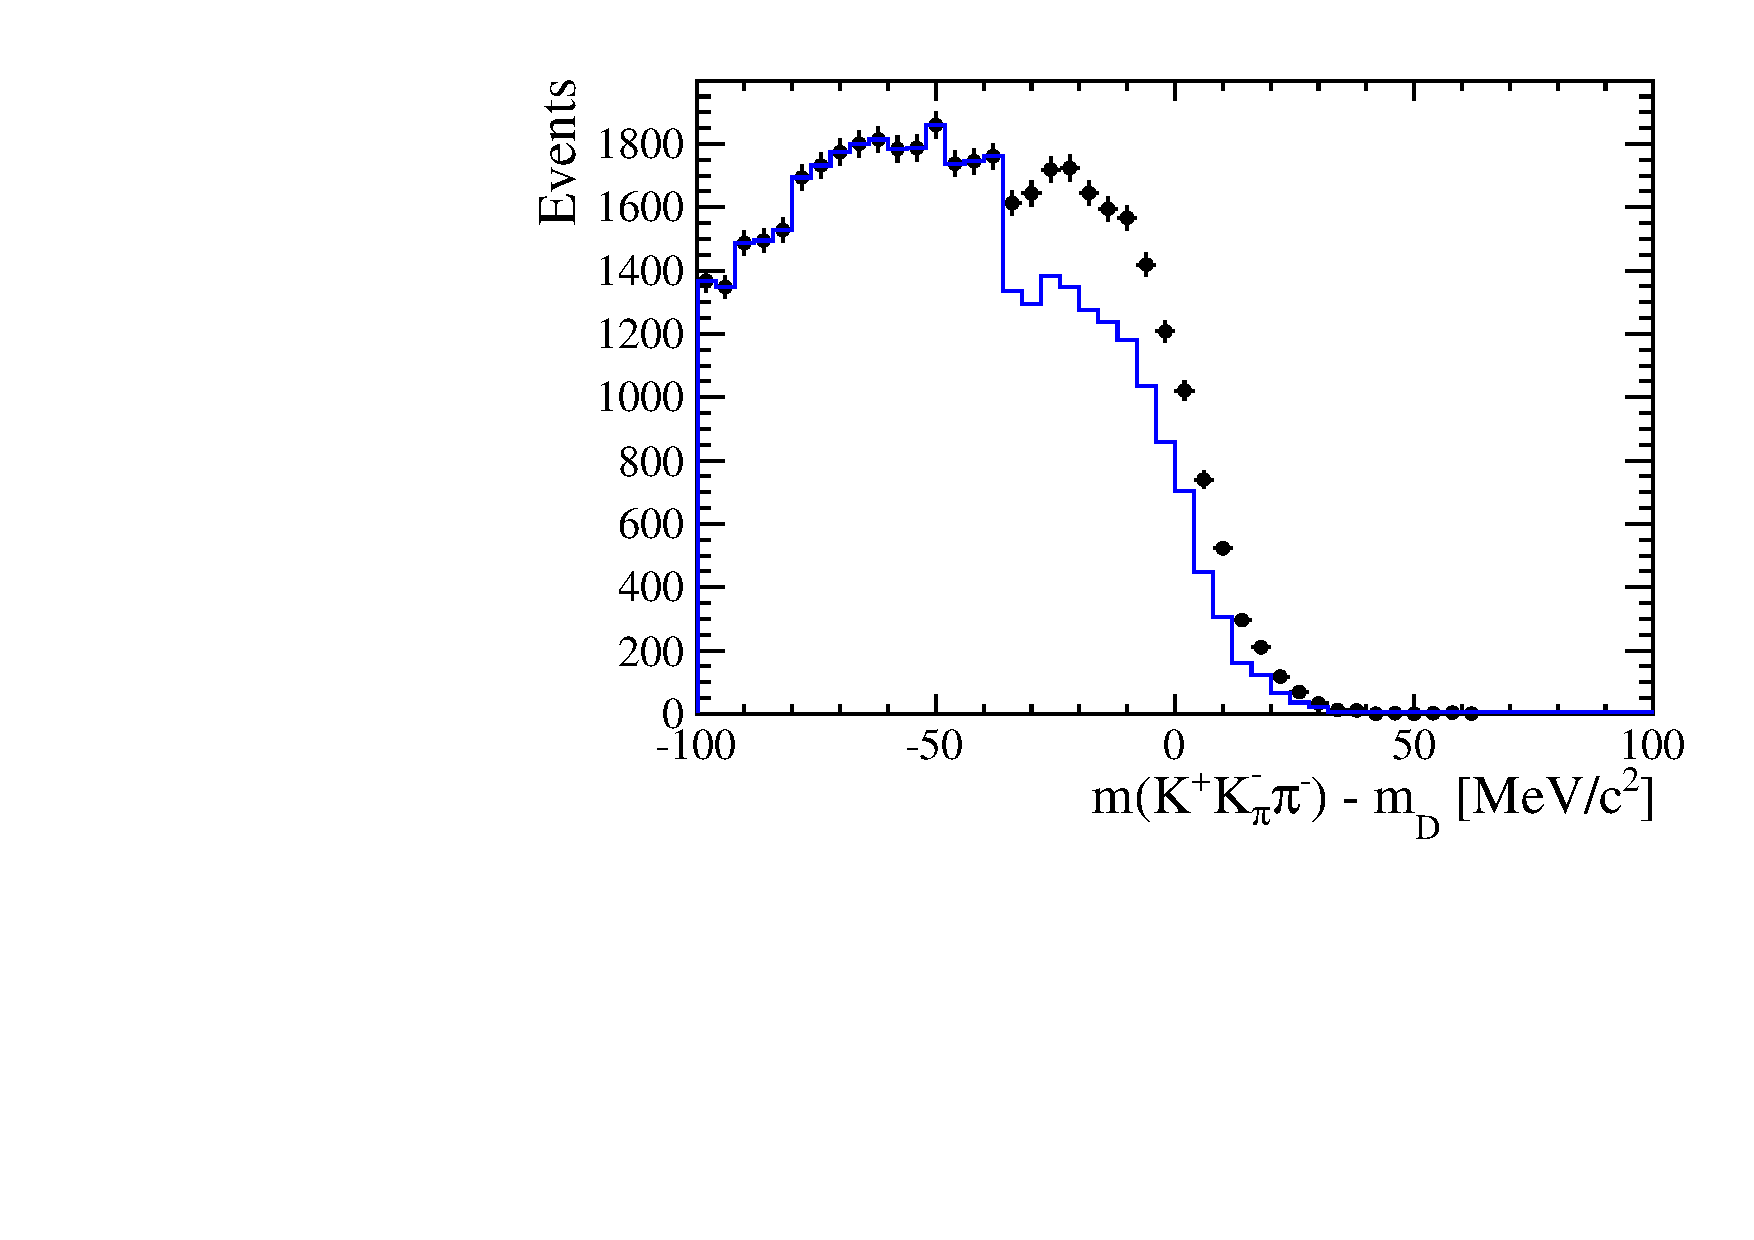
\includegraphics[height=!,width=0.32\textwidth]{figs/BkgStudies/norm_Ds2KKpi_as_D2Kpipi_compareVeto_0.pdf} 
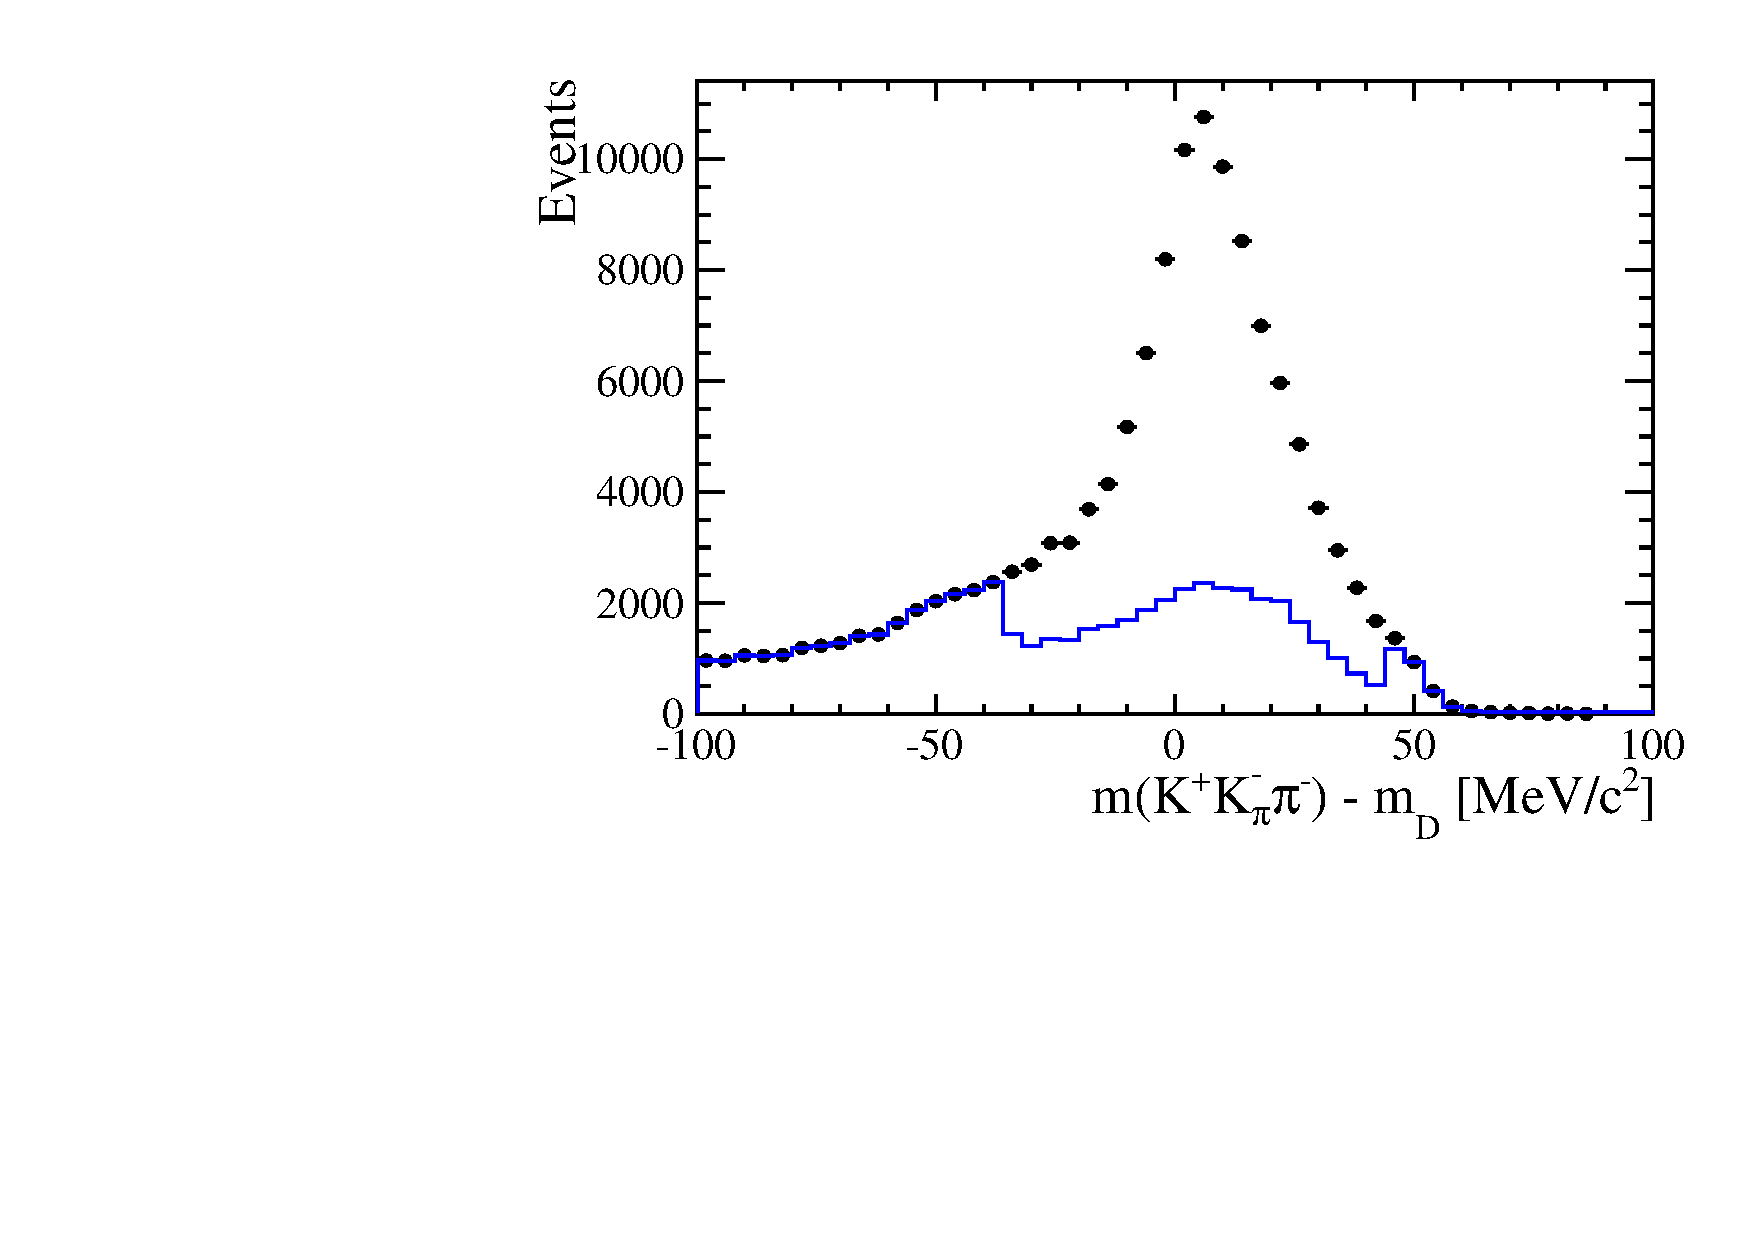
\includegraphics[height=!,width=0.32\textwidth]{figs/BkgStudies/norm_Ds2KKpi_as_D2Kpipi_compareVeto_1.pdf}

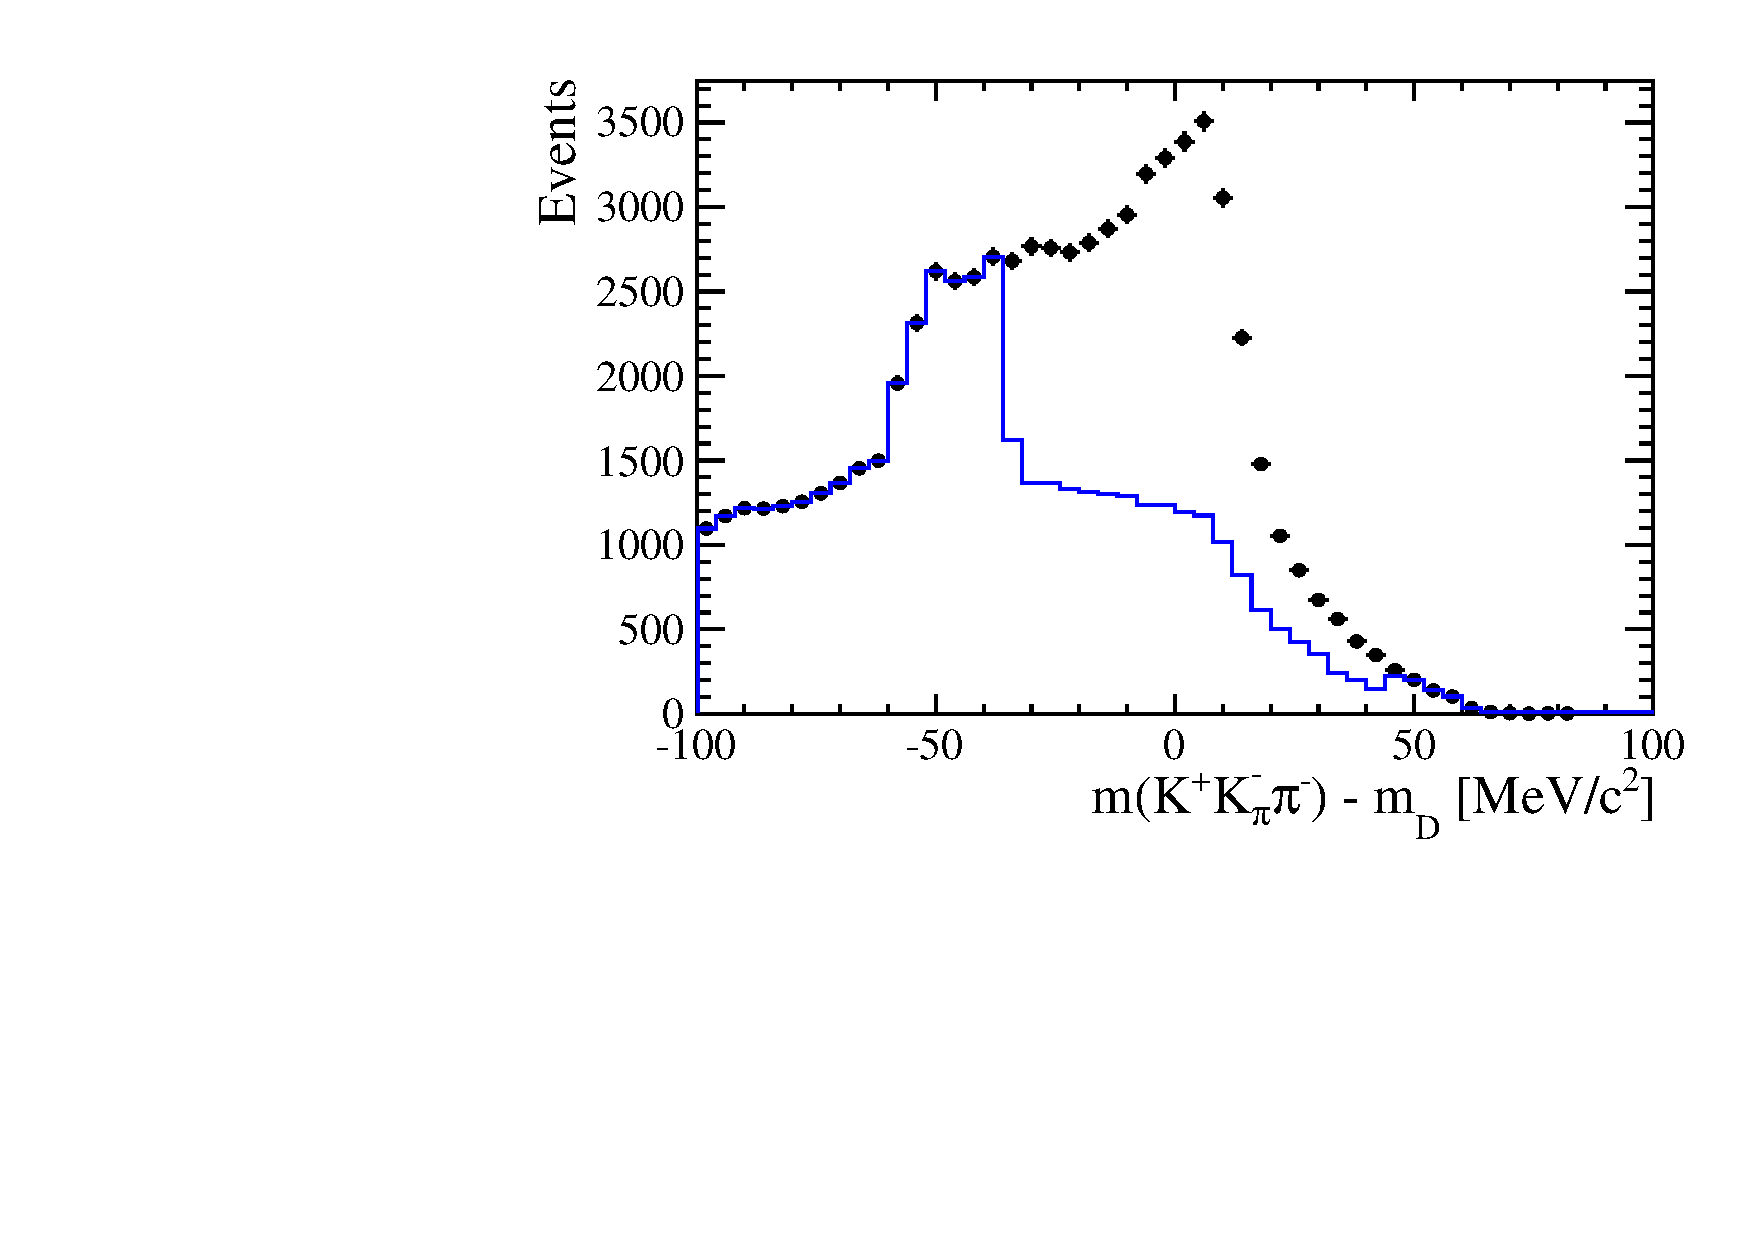
\includegraphics[height=!,width=0.32\textwidth]{figs/BkgStudies/norm_Ds2KKpi_as_D2Kpipi_compareVeto_2.pdf} 
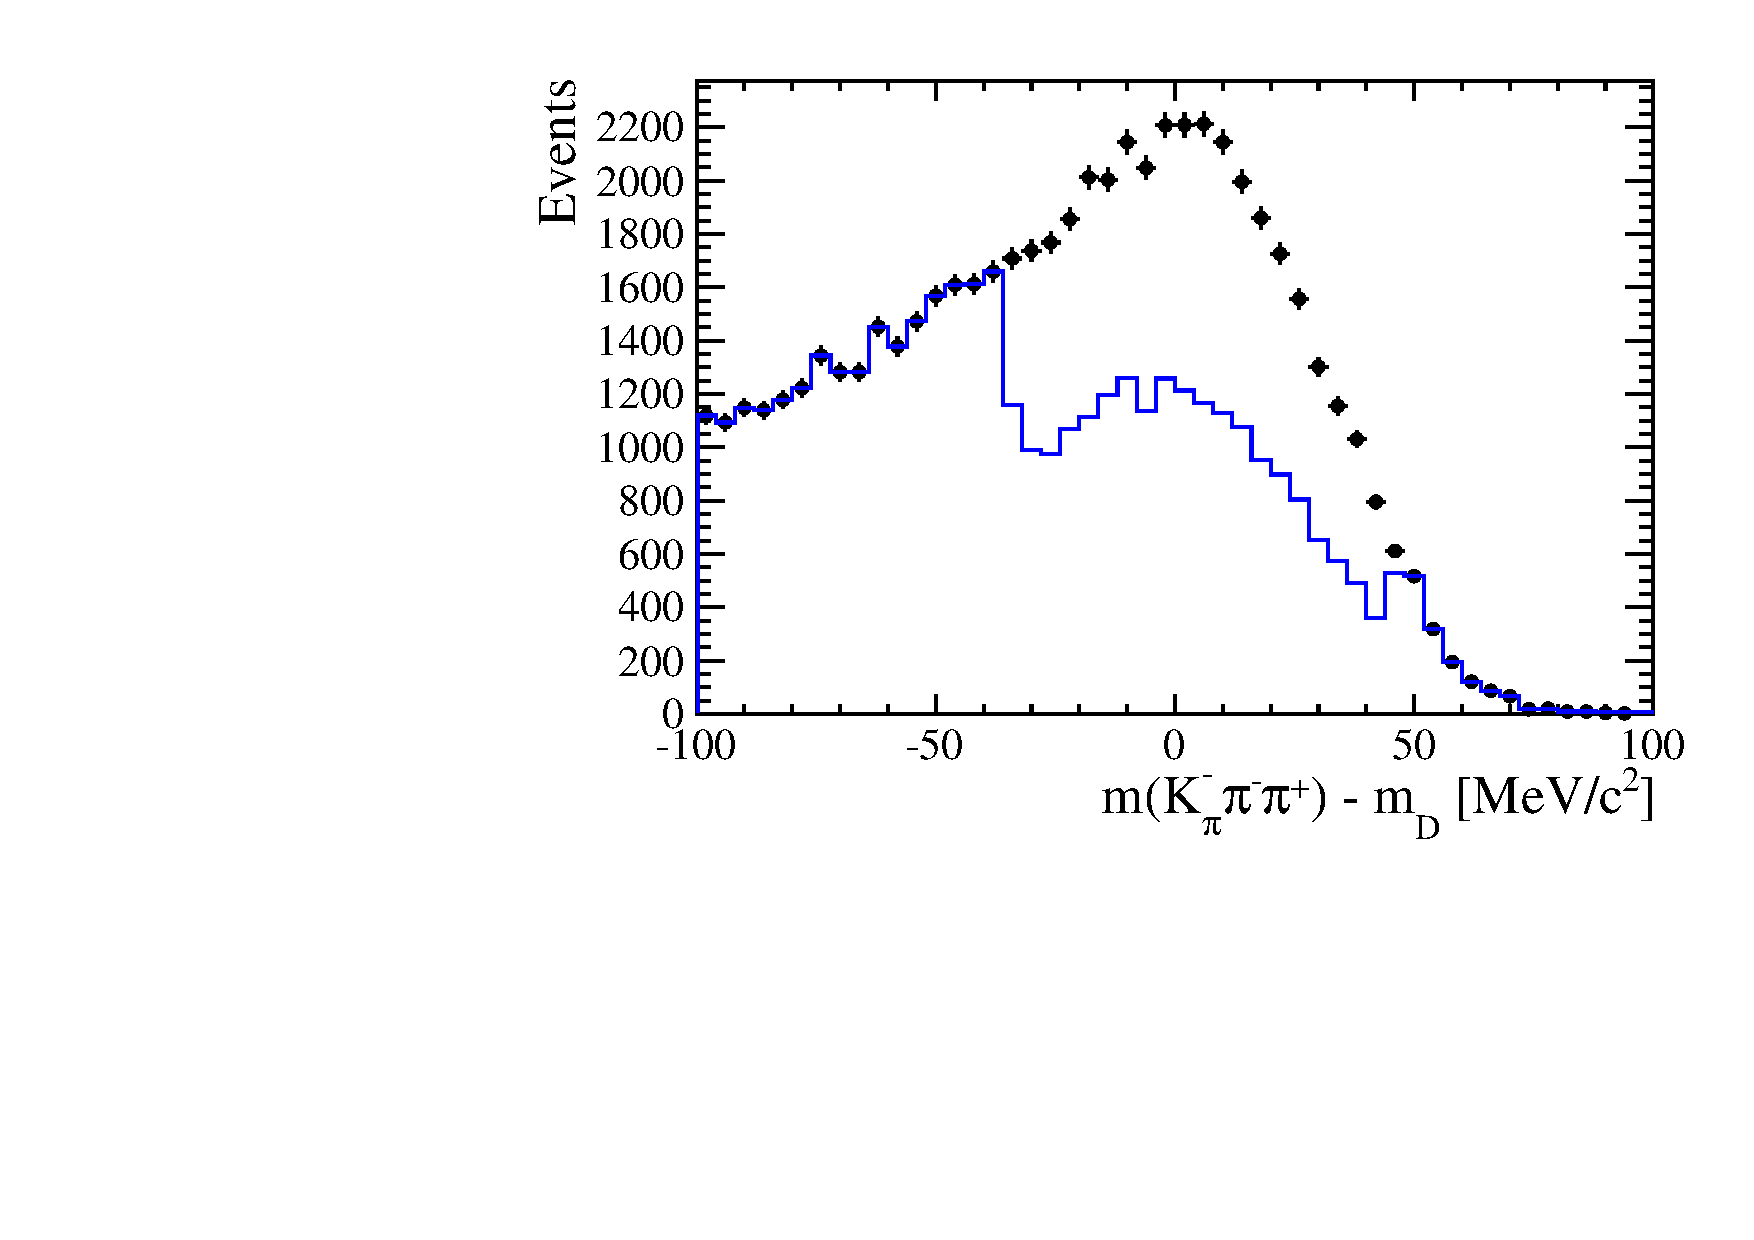
\includegraphics[height=!,width=0.32\textwidth]{figs/BkgStudies/norm_Ds2Kpipi_as_D2pipipi_compareVeto.pdf}
\caption{
Background contributions from $D^-$ decays where the $\pim$ is misidentified as $\Km$. 
The $D_s$ invariant mass is recomputed applying the pion mass hypothesis to the kaon and shown for the 
$D_s \to \phi \pi$, $D_s \to K^*(892)K$, $D_s \to KK\pi$ (non-resonant) and $D_s \to K\pi\pi$ final state categories
from top-left to bottom-right.
The distributions are shown without (black) and with (blue) the $D^-$-veto applied. 
%The $B_s \to D_s \pi\pi\pi$ sample passing all selection cuts listed in Tables \ref{table:selDs} and \ref{table:selBs} except for the 
}
\label{fig:vetoD}
\end{figure}
%
\begin{figure}[h]
\centering
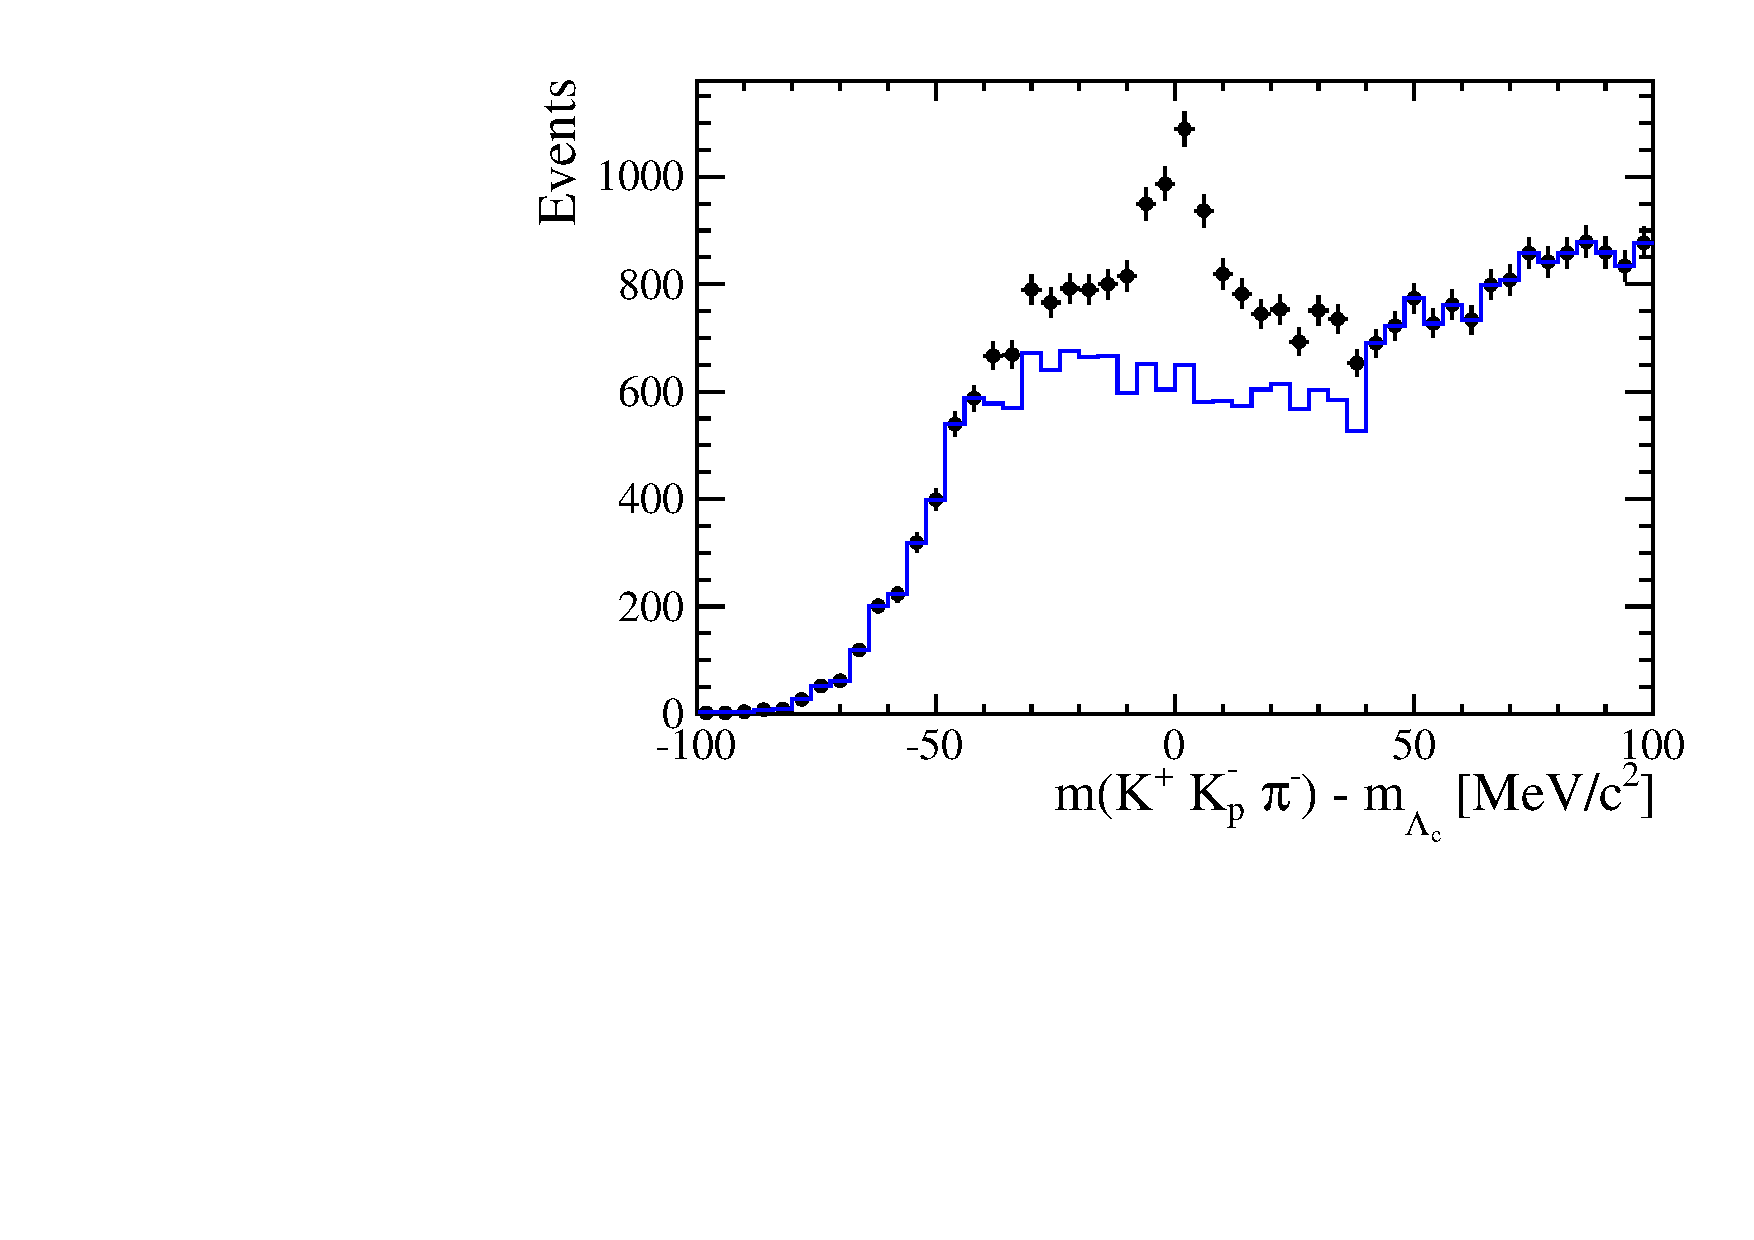
\includegraphics[height=!,width=0.32\textwidth]{figs/BkgStudies/norm_Ds2KKpi_as_Lc2KPpi_compareVeto_0.pdf} 
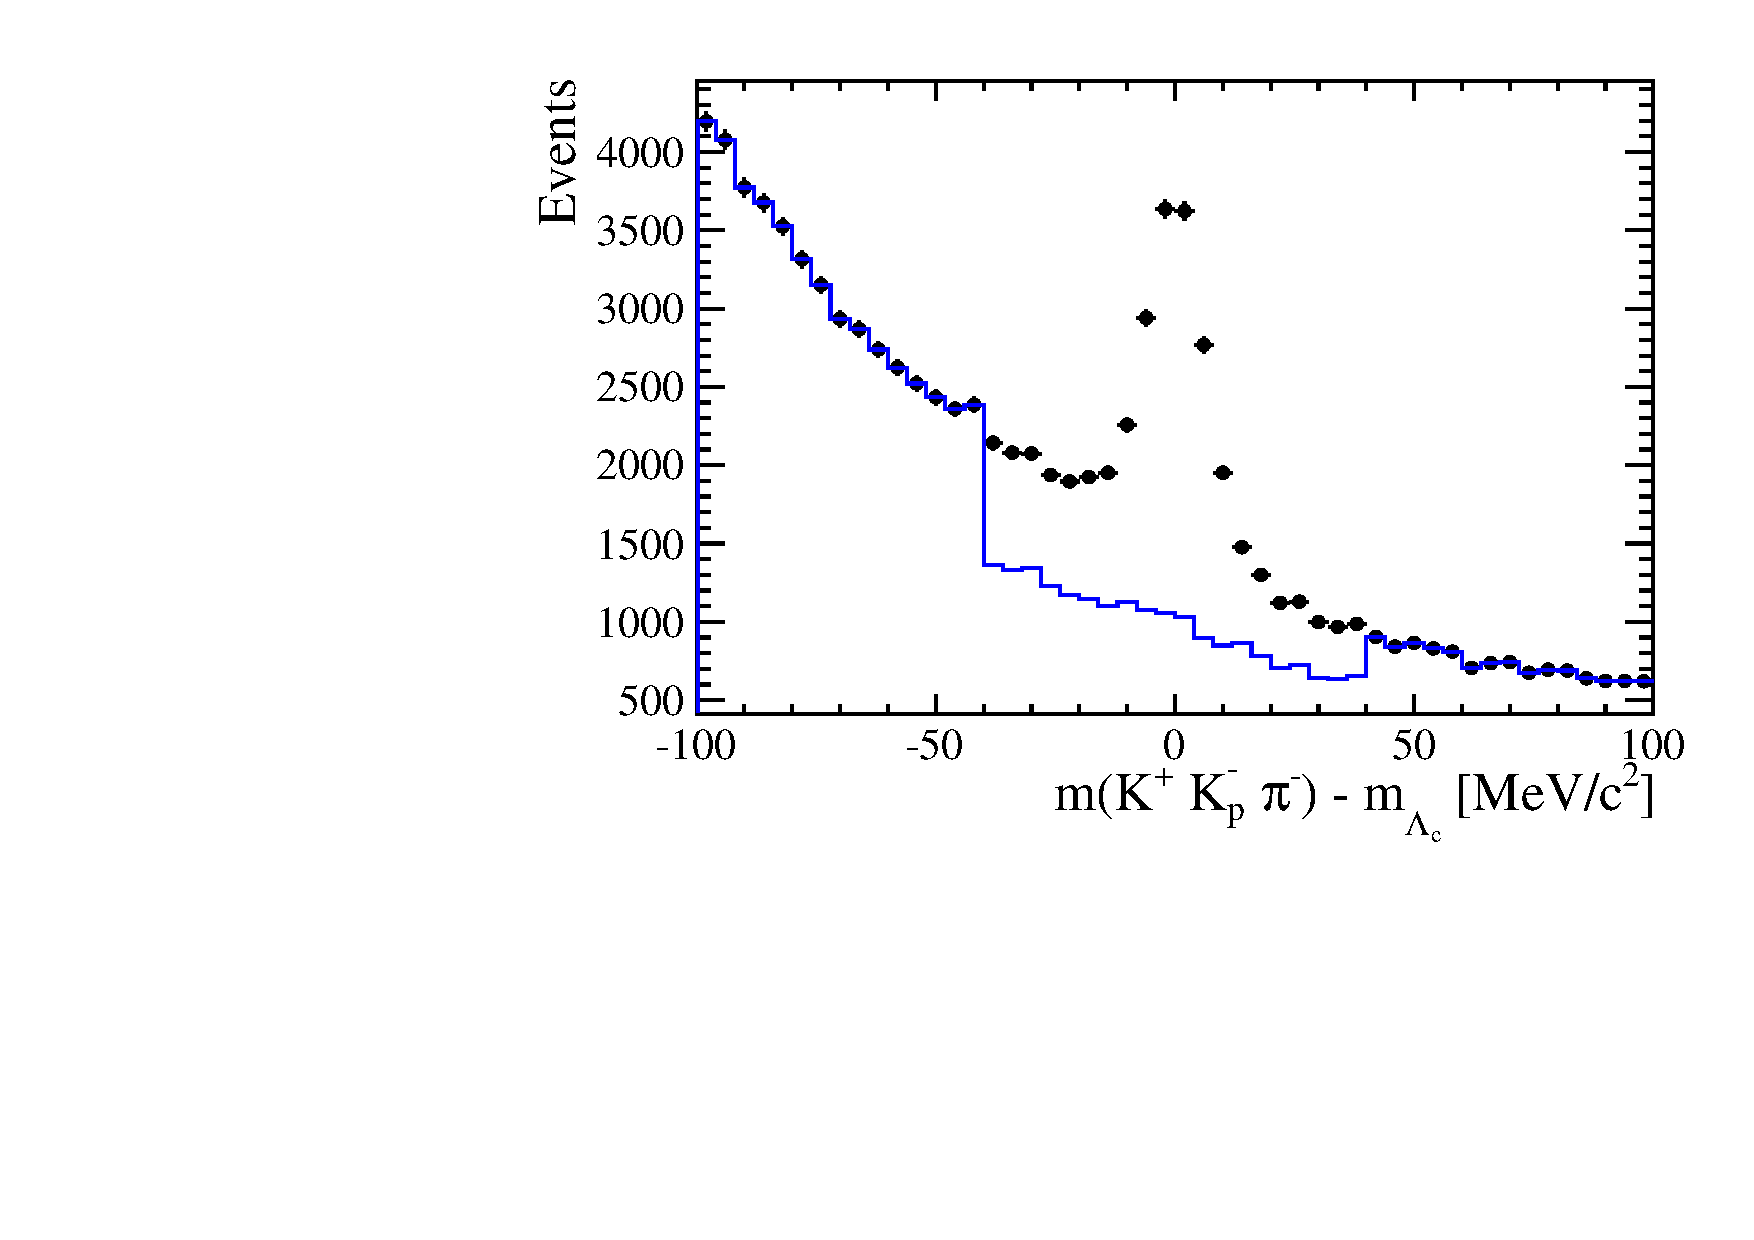
\includegraphics[height=!,width=0.32\textwidth]{figs/BkgStudies/norm_Ds2KKpi_as_Lc2KPpi_compareVeto_1.pdf}

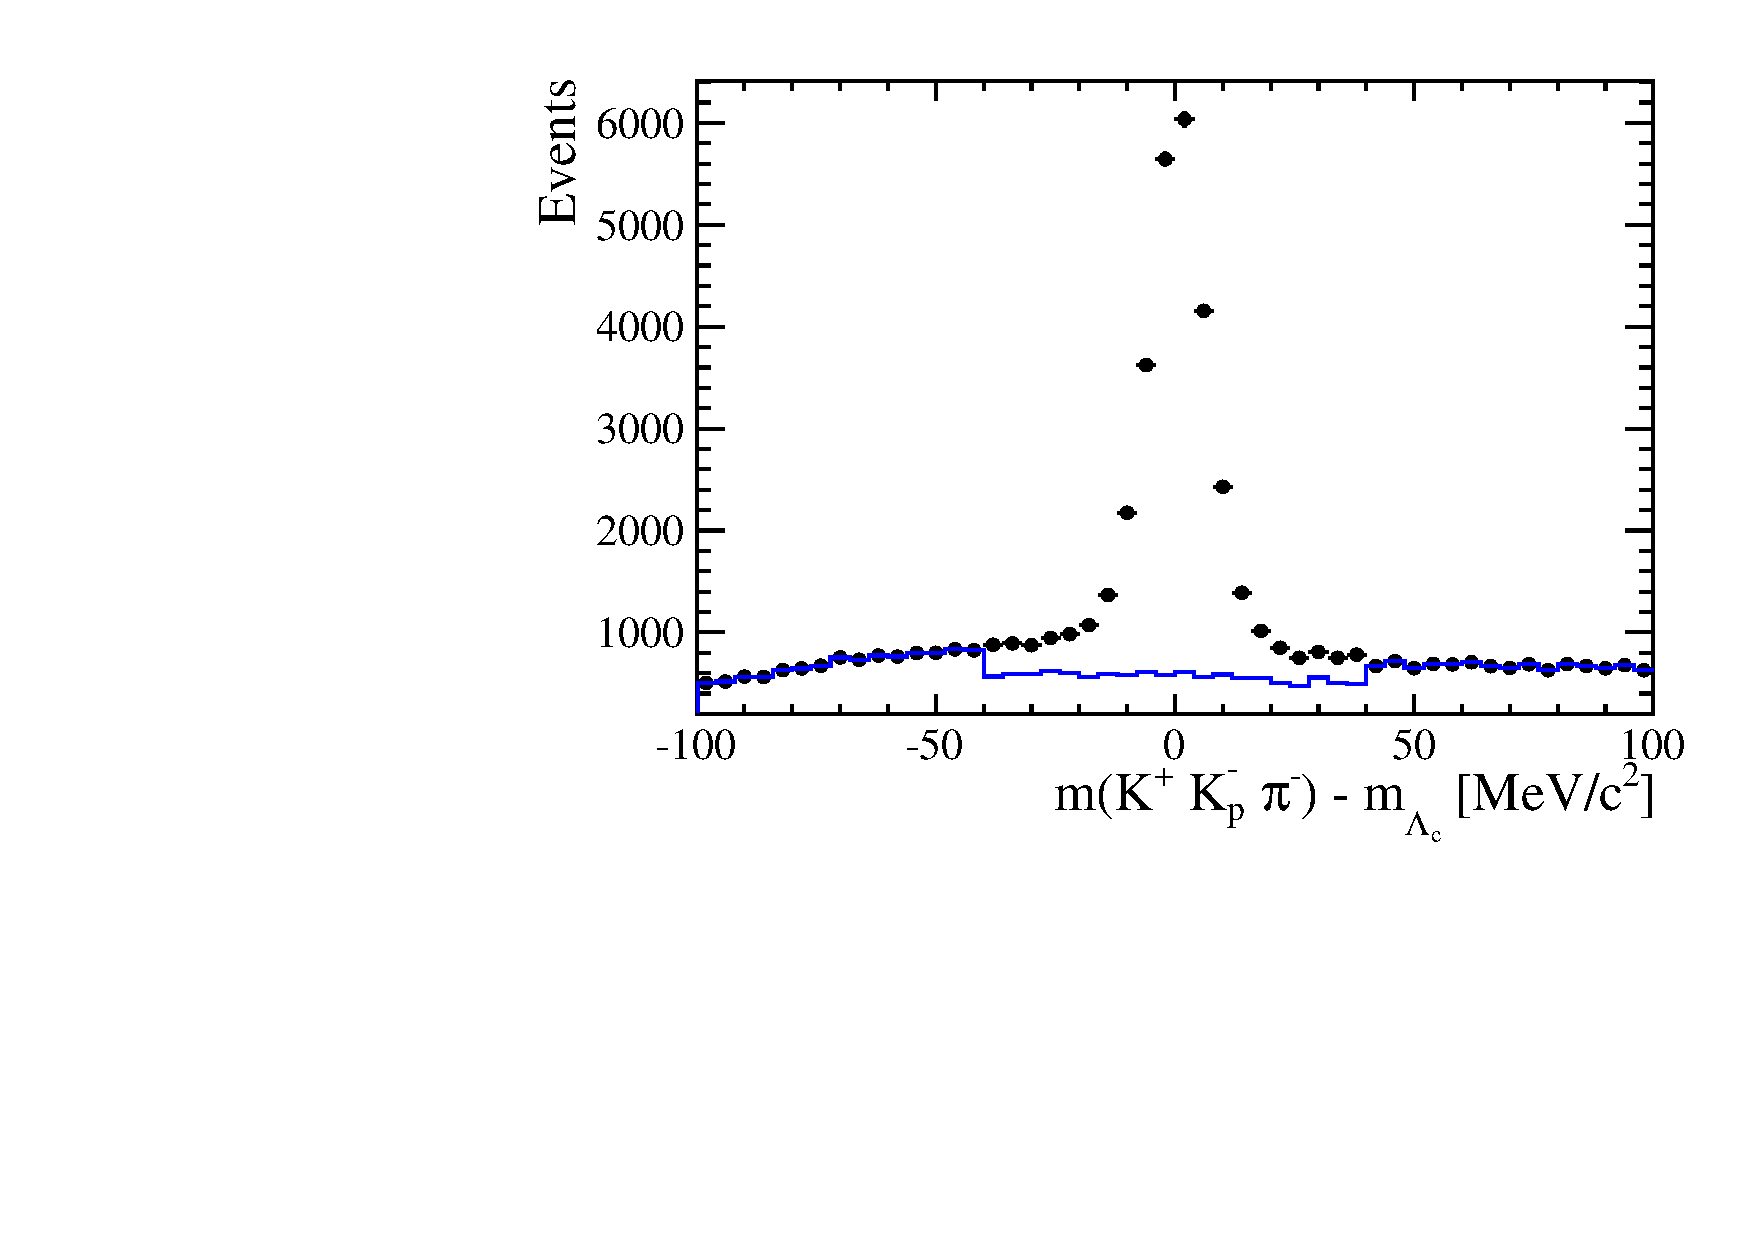
\includegraphics[height=!,width=0.32\textwidth]{figs/BkgStudies/norm_Ds2KKpi_as_Lc2KPpi_compareVeto_2.pdf} 
%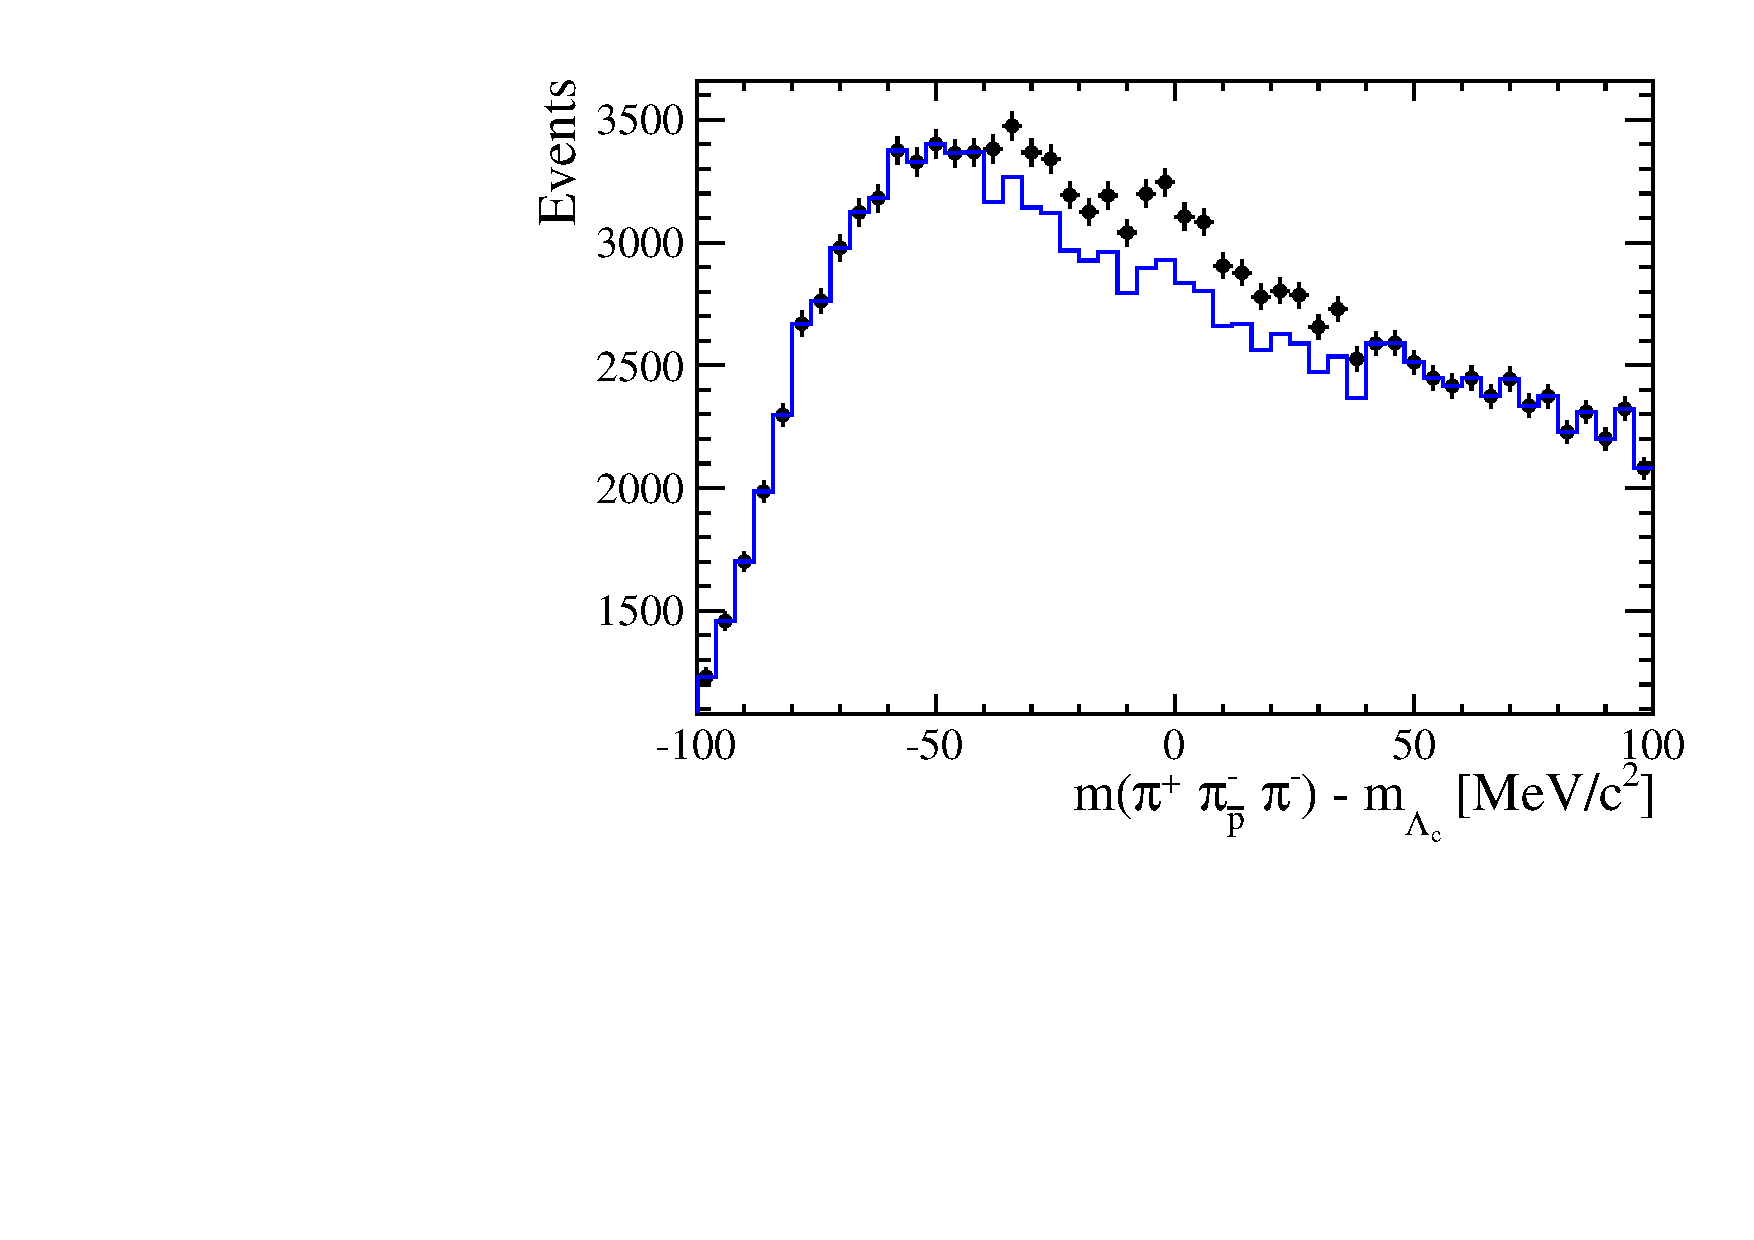
\includegraphics[height=!,width=0.32\textwidth]{figs/BkgStudies/norm_Ds2pipipi_as_Lc2piPpi_compareVeto.pdf}
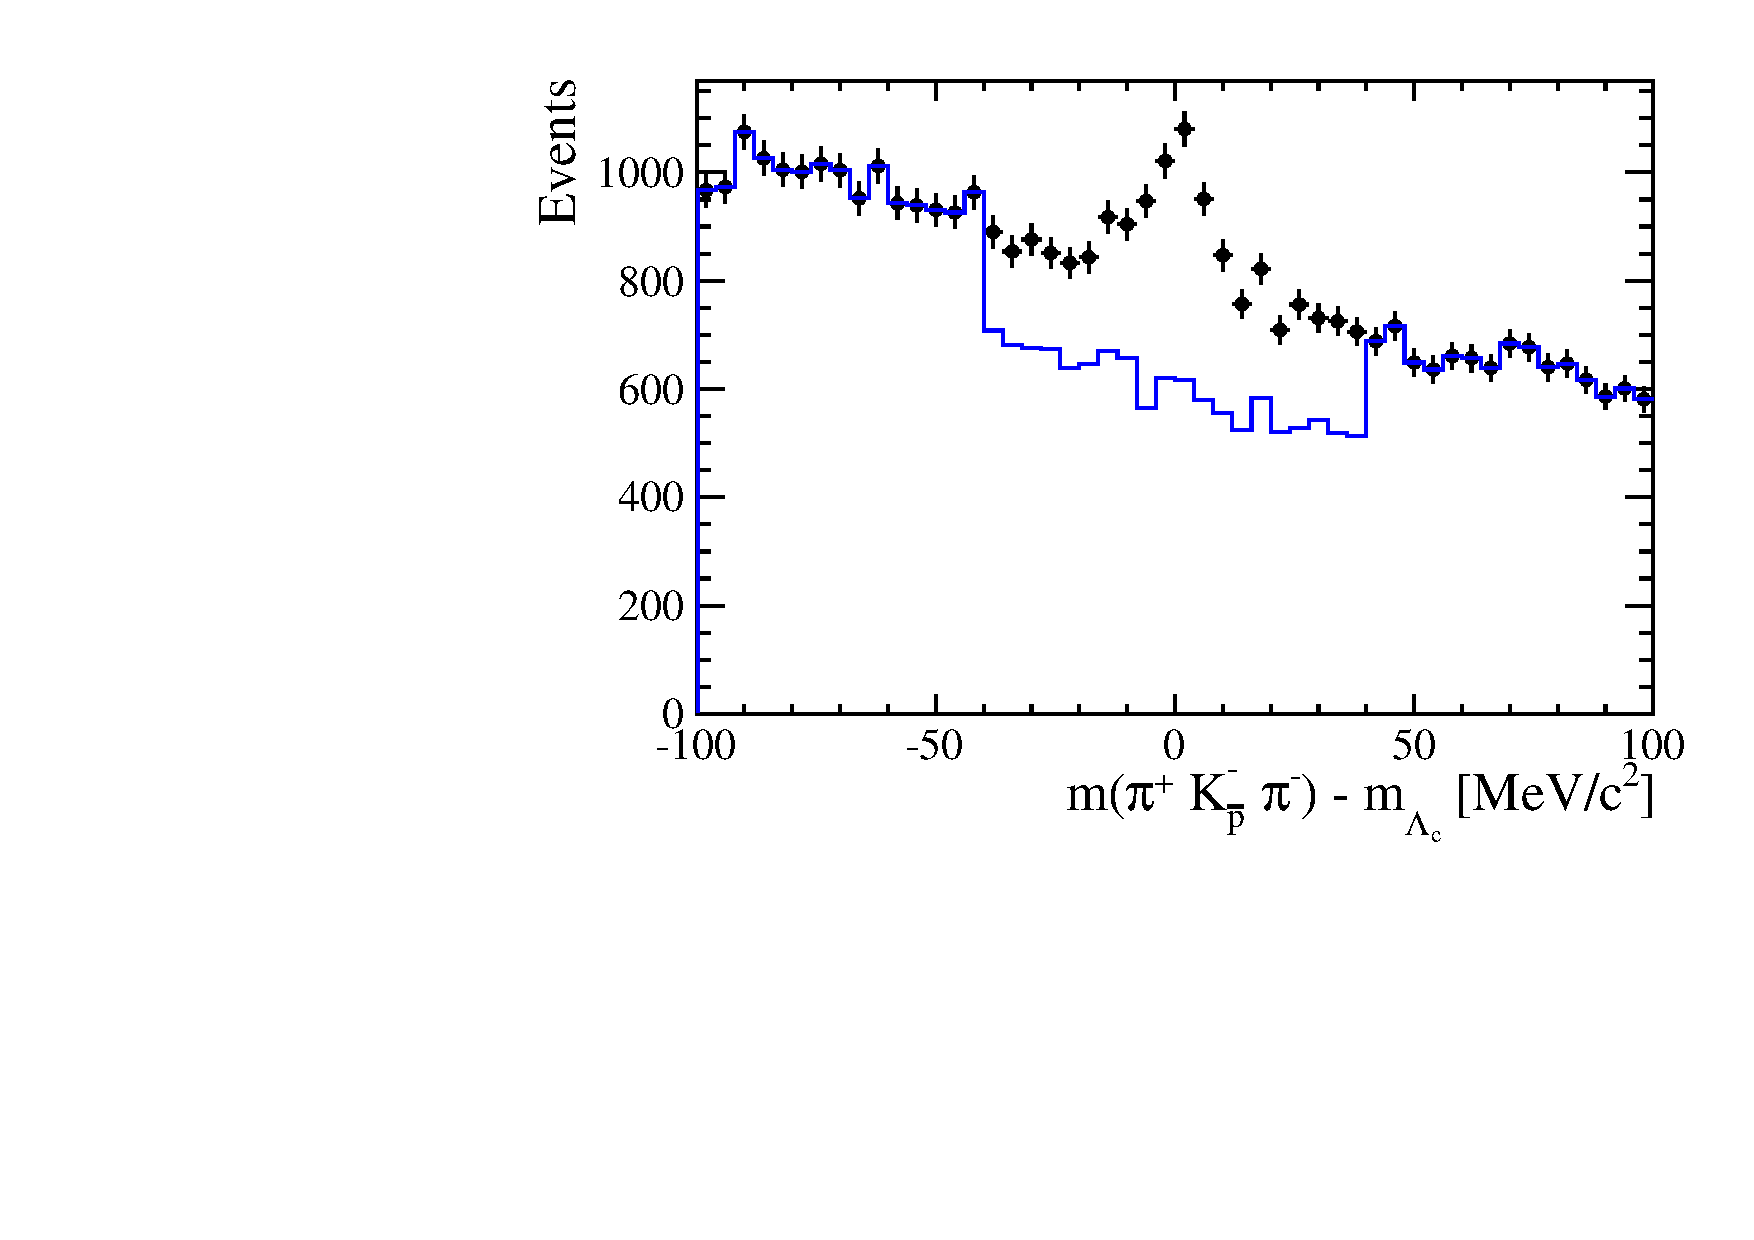
\includegraphics[height=!,width=0.32\textwidth]{figs/BkgStudies/norm_Ds2Kpipi_as_Lc2piPpi_compareVeto.pdf}
\caption{Background contributions from $\Lambda_c$ decays where the $\bar p$ is misidentified as $\Km$. 
The $D_s$ invariant mass is recomputed applying the proton mass hypothesis to the kaon and shown for the 
$D_s \to \phi \pi$, $D_s \to K^*(892)K$, $D_s \to KK\pi$ (non-resonant) and $D_s \to K\pi\pi$ final state categories
from top-left to bottom-right.
The distributions are shown without (black) and with (blue) the $\Lambda_c$-veto applied.}
\label{fig:vetoLambda}
\end{figure}
\begin{figure}[h]
\centering
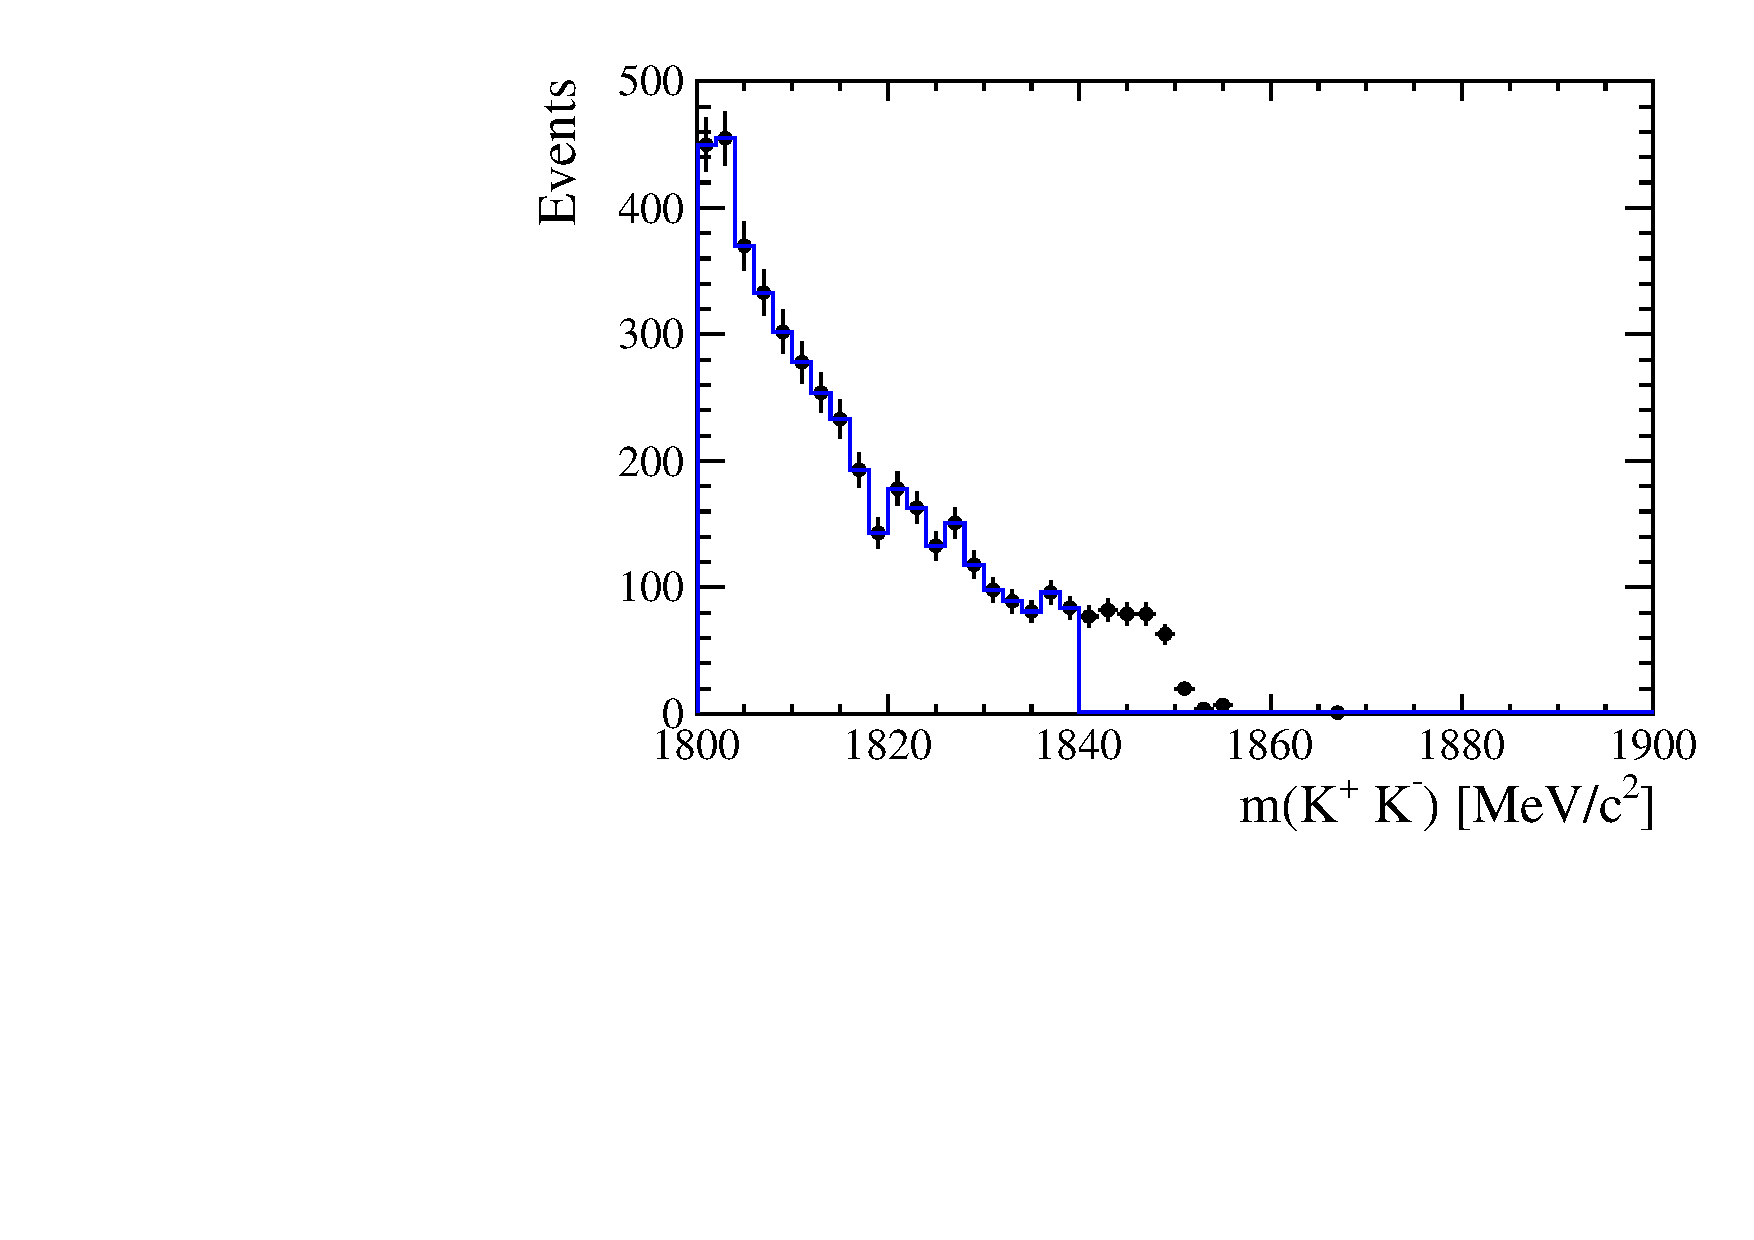
\includegraphics[height=!,width=0.32\textwidth]{figs/BkgStudies/norm_Ds2KKpi_as_D02KK_compareVeto.pdf} 
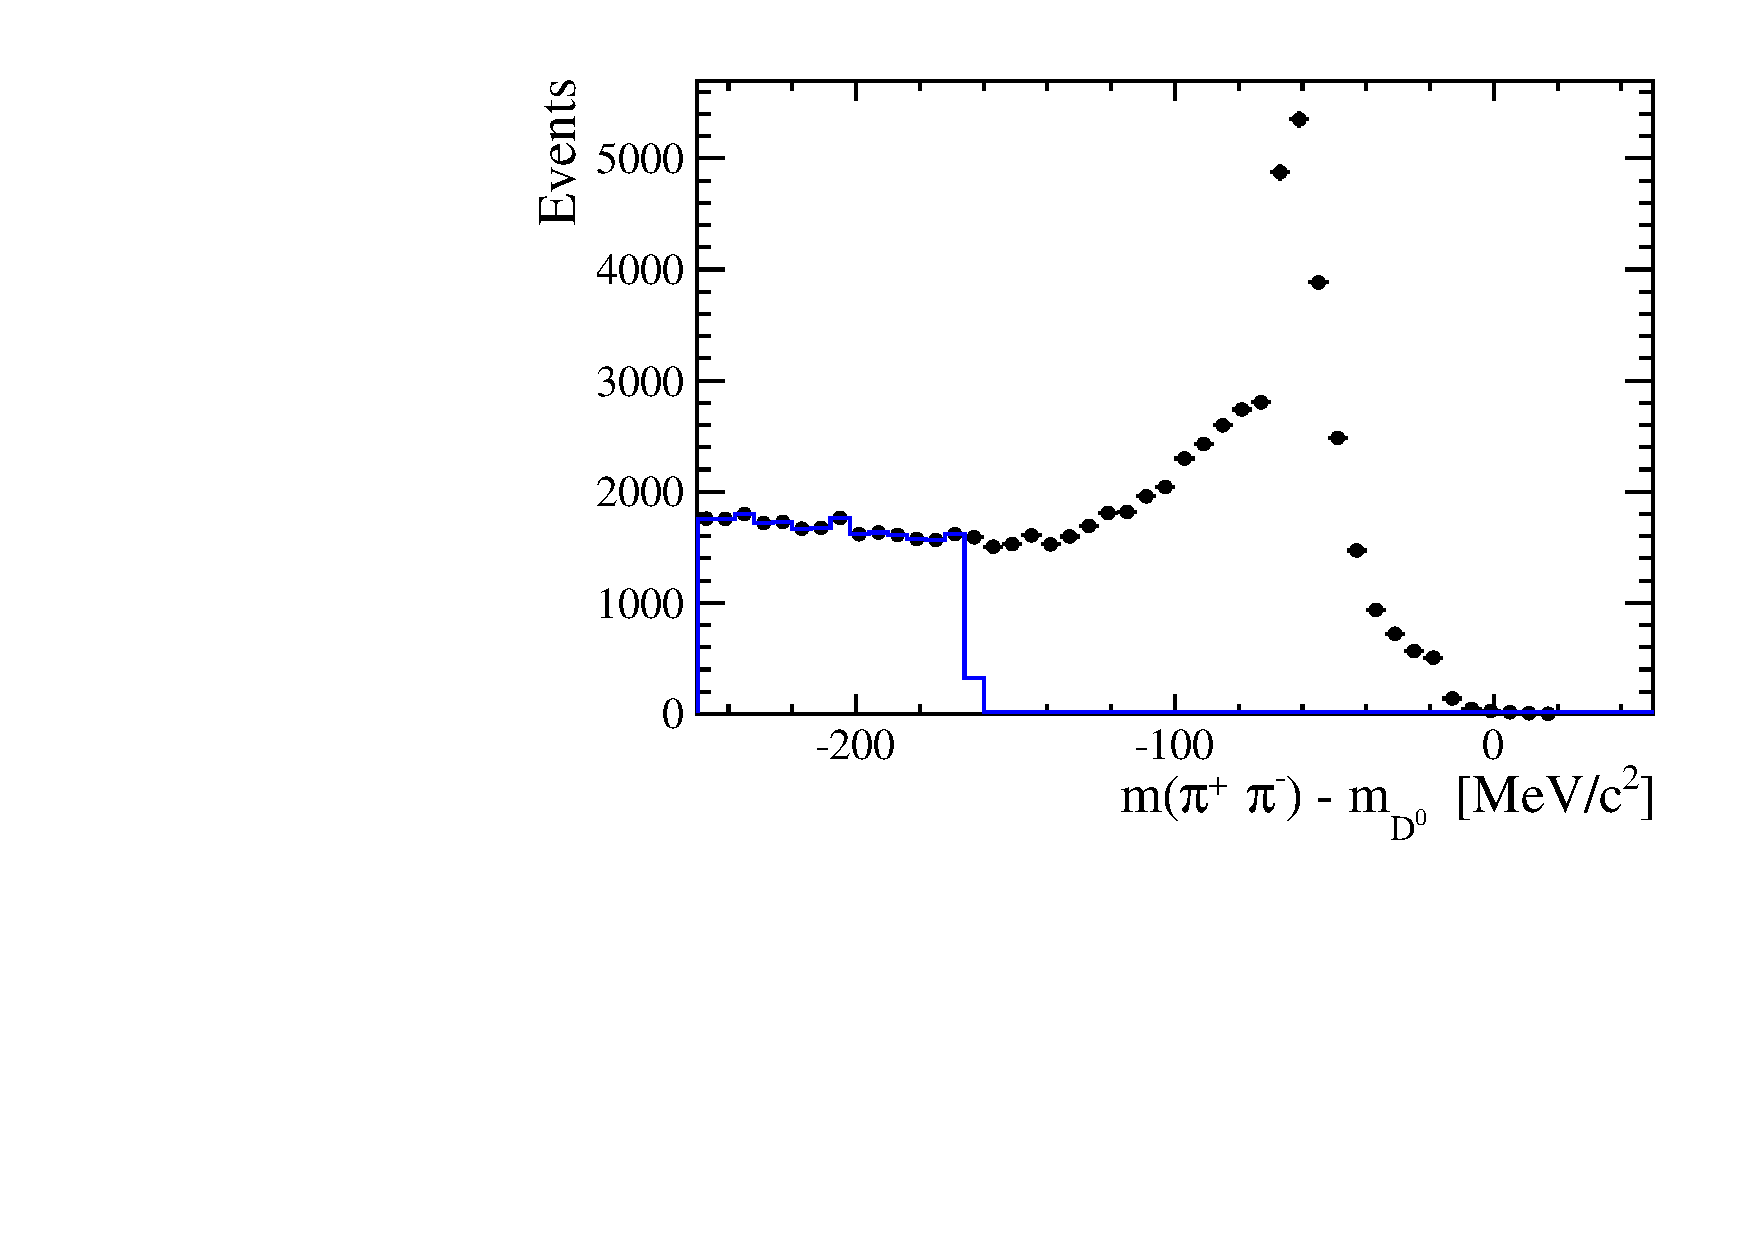
\includegraphics[height=!,width=0.32\textwidth]{figs/BkgStudies/norm_Ds2pipipi_as_D02pipi_compareVeto.pdf} 
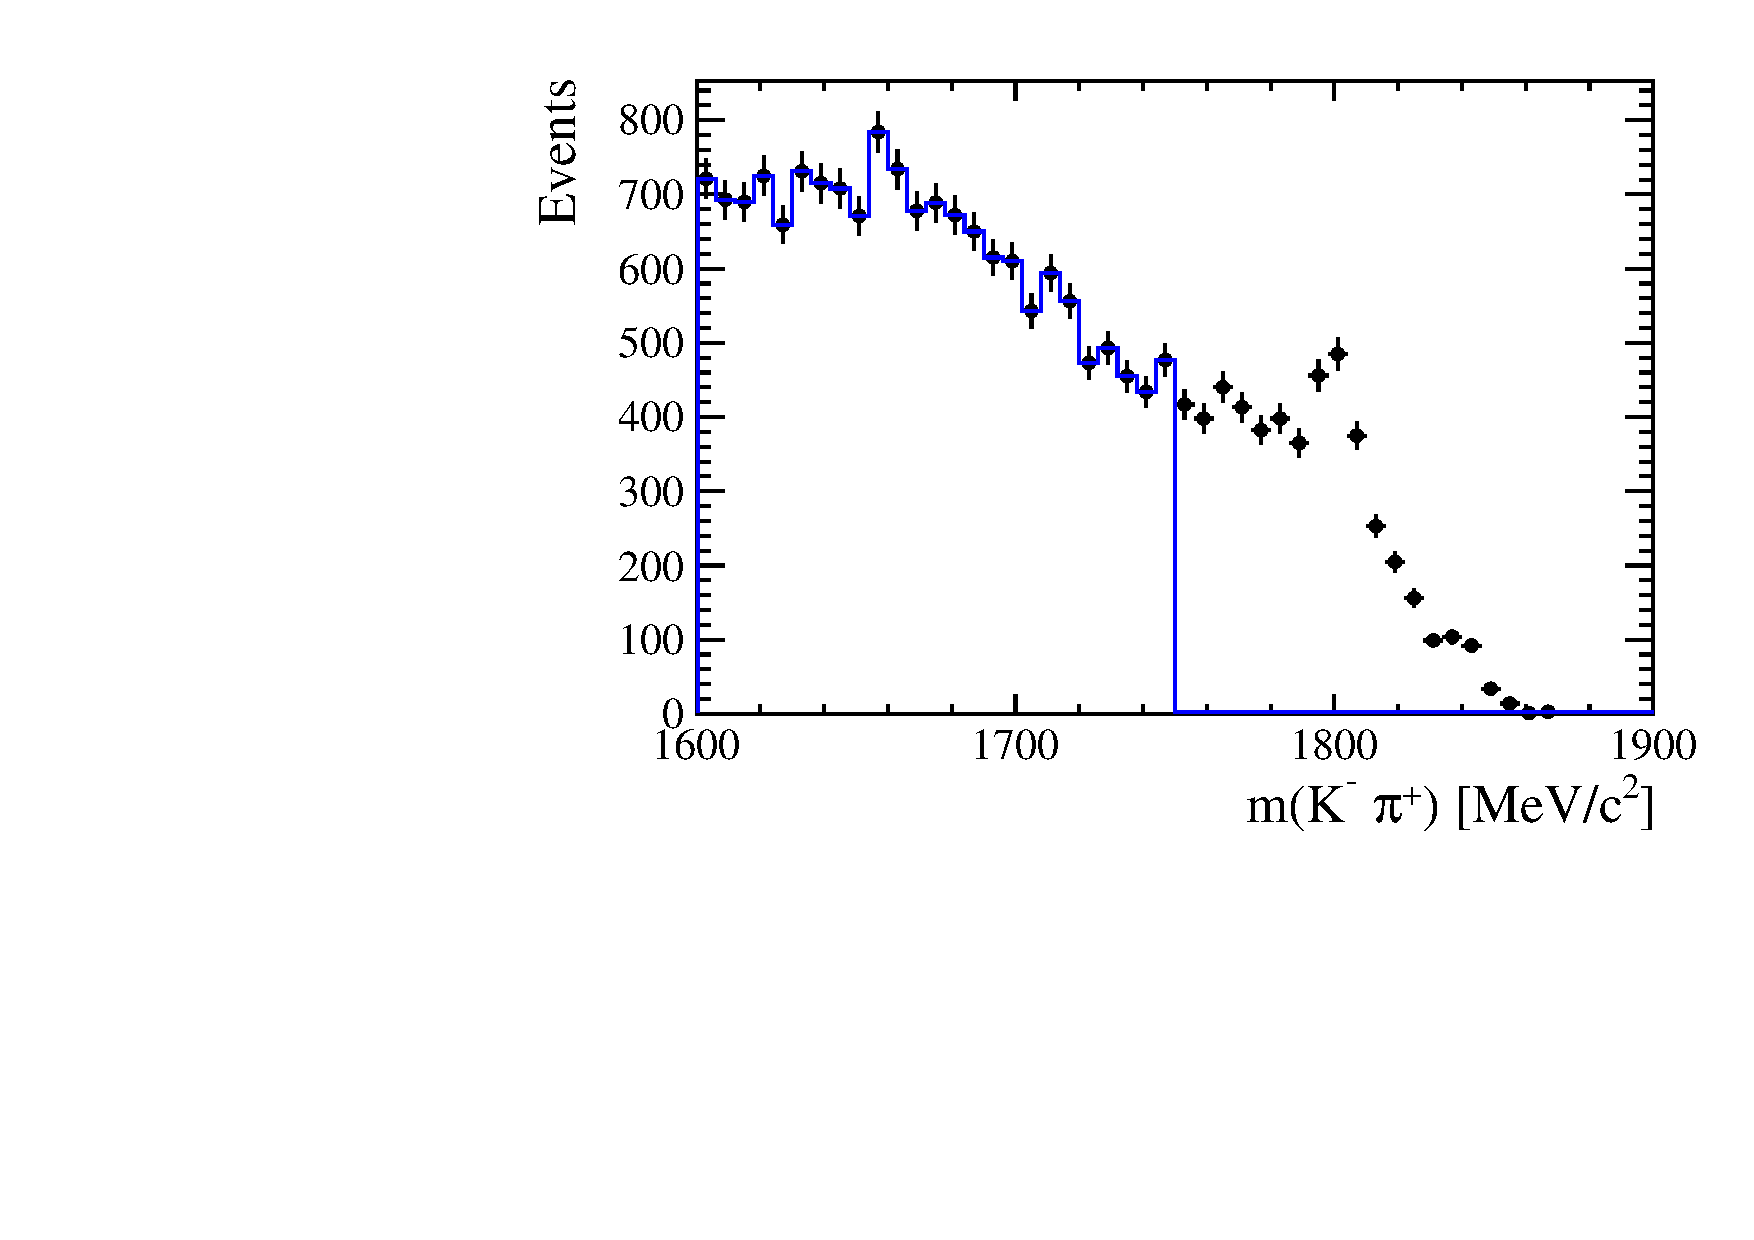
\includegraphics[height=!,width=0.32\textwidth]{figs/BkgStudies/norm_Ds2Kpipi_as_D02Kpi_compareVeto.pdf} 
\caption{
Background contributions to $D_s \to KK\pi$ (left), $D_s \to \pi\pi\pi$ (middle) and $D_s \to K\pi\pi$ (right) from $D^0\to hh$ decays combined with a random pion.
The peak at $m(\pi\pi) - m(D^0) \approx -60 \mev$ ($m(K\pi) - m(D^0) \approx -60 \mev$) are due to $D^0\to K\pi$ ($D^0\to KK$) where a kaon is misidentified as pion.
%Background contributions to $D_s^- \to KK\pi$ (left), $D_s^- \to \pi\pi\pi$ (middle) and $D_s^- \to K\pi\pi$ (right) from $D^{*-} \to (D^0\to hh) \pim$ decays. 
%The $D^{*-}$ background contribution peaks at $m(hh\pim) - m(hh) \approx 145.5 \mev$ which corresponds to the mass difference of the $D^{*-}$ and $D^0$ mesons. 
}
\label{fig:vetoD0}
\end{figure}
\begin{figure}[h]
\centering
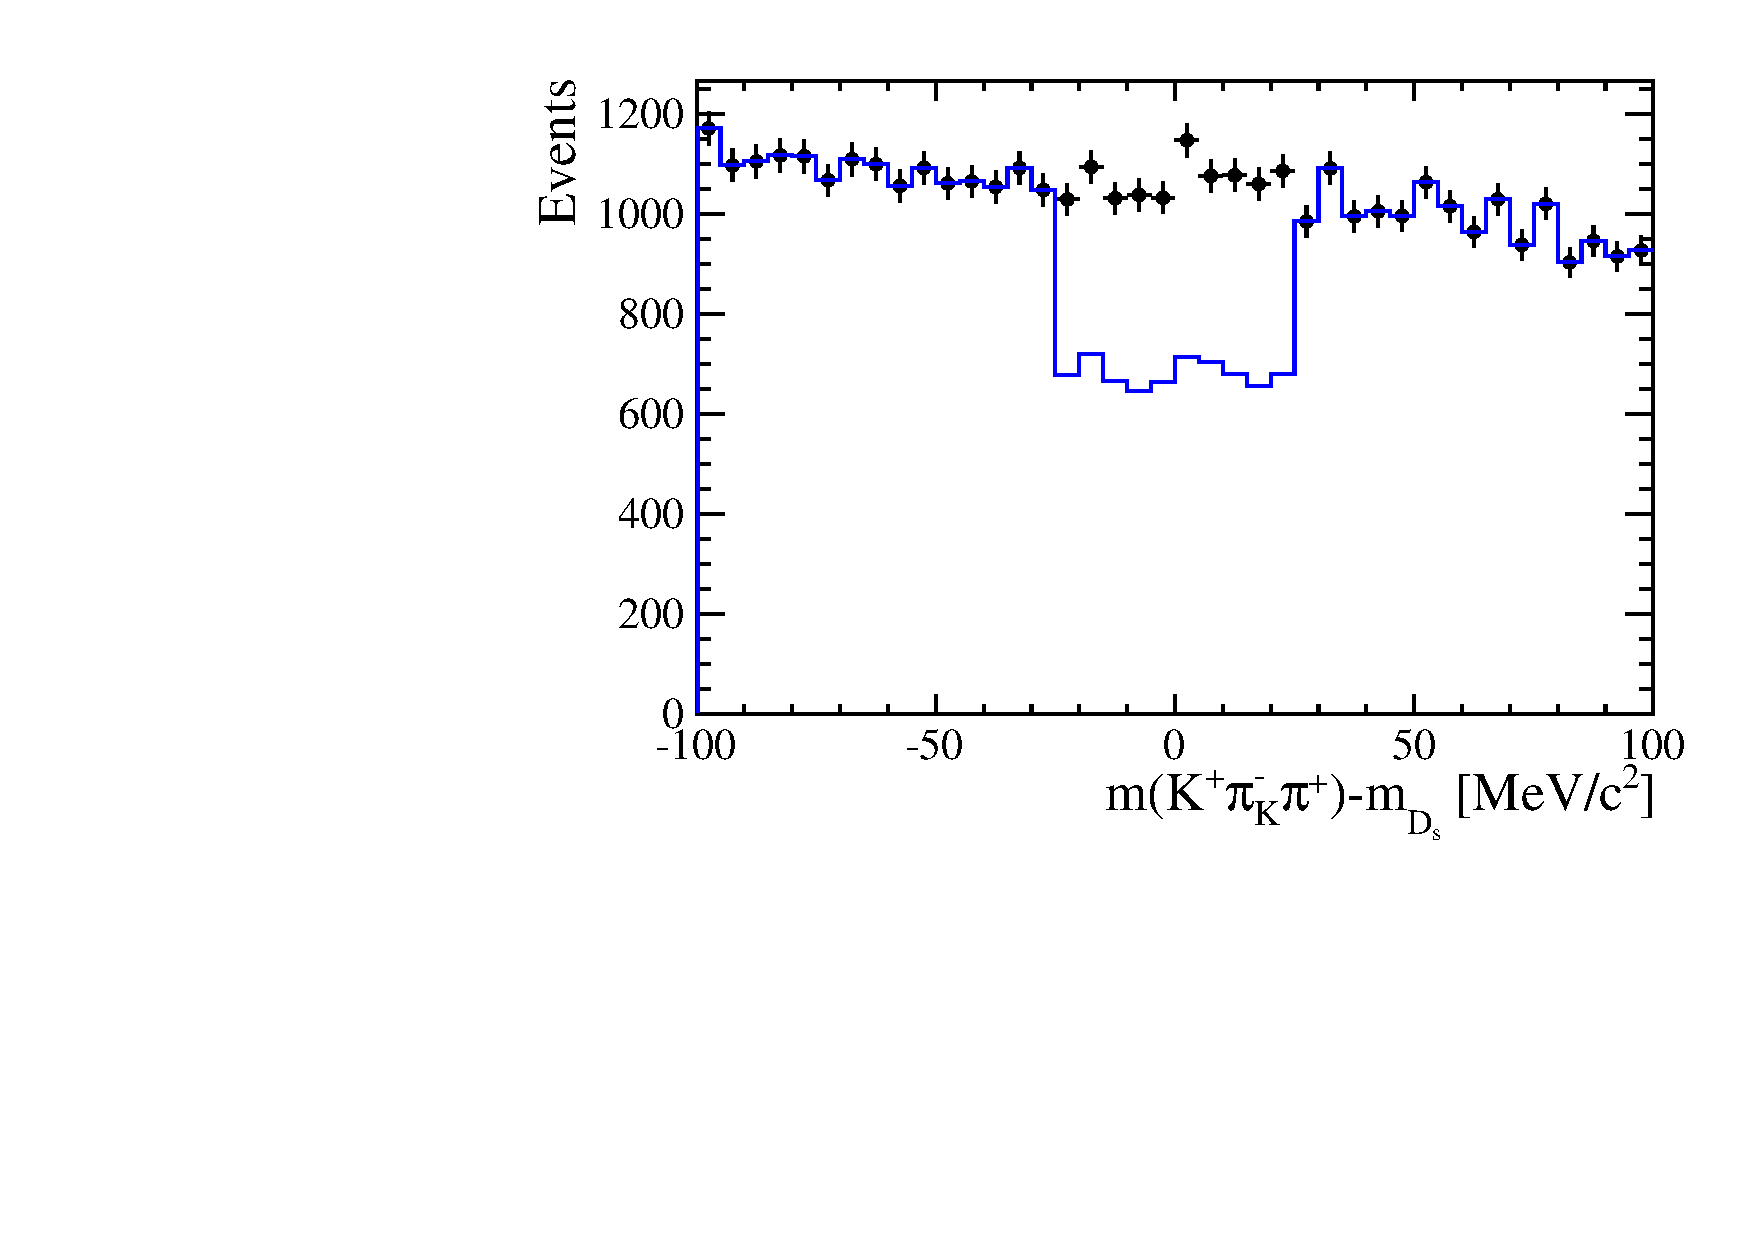
\includegraphics[height=!,width=0.32\textwidth]{figs/BkgStudies/signal_Bs2DsKpipi_as_Bs2DsDs_compareVeto.pdf} 
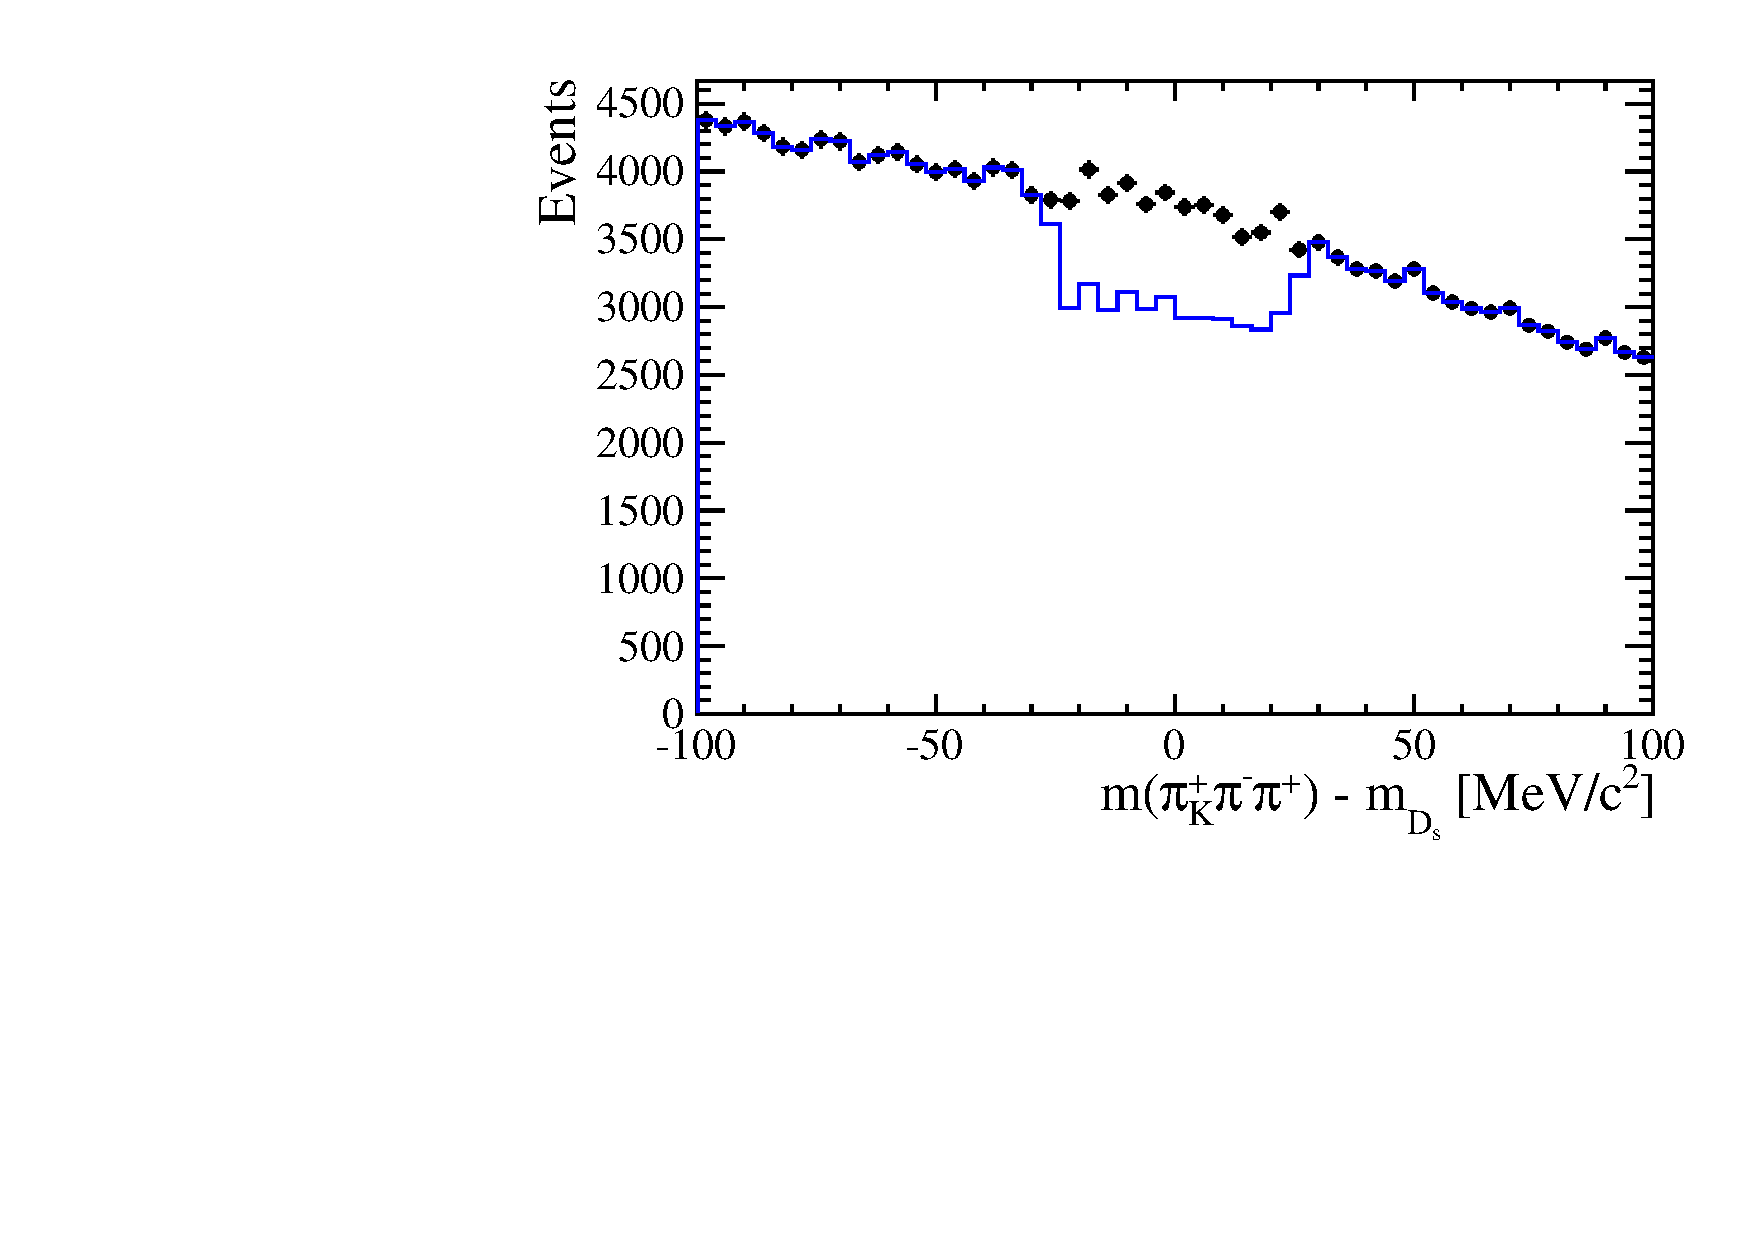
\includegraphics[height=!,width=0.32\textwidth]{figs/BkgStudies/norm_Bs2Dspipipi_as_Bs2DsDs_compareVeto.pdf} 
\caption{Background contributions to  $B_s \to D_s K\pi\pi$ (left) and $B_s \to D_s \pi\pi\pi$ (right) from $B_s \to D_s D_s$ decays where the kaon is misidentified as pion.
The $X_{s,d}$ invariant mass is recomputed applying the kaon mass hypothesis to the pion and shown without (black) and with (blue) the $D_s$-veto applied. 
}
\label{fig:vetoDs}
\end{figure}



\clearpage
\subsubsection{Training of multivariate classifier}

The Toolkit for Multivariate Analysis (TMVA \cite{Hocker:2007ht}) is used to train a multivariate classifier (BDT with gradient boosting, BDTG)
discriminating signal and combinatorial background.
We use $B_s\to D_s\pi\pi\pi$ data that passes all previously mentioned selection steps, including the trigger and stripping selection, offline cuts and physical background vetoes, 
as signal proxy. 
The background is statistically subtracted by applying \textsf{sWeights} based on the fit to the reconstructed $B_s$ mass shown in Fig.~\ref{fig:massFit_preselected}(left).
This is a simplified version (performed in a reduced mass range) of the final mass fits described in Sec.~\ref{sec:massFits}.
The sideband  $B_s\to D_sK\pi\pi$ data ($m(B_s) > 5500 \mev$) is used as background proxy.

Training the classifier on a sub-sample which is supposed to be used in the
final analysis might cause a bias, as the classifier selects, in case of overtraining,  the training events more efficiently. 
As overtraining can not be completely avoided, we split the signal and
the background training samples into two disjoint subsamples according to whether the
event number is even or odd. We then train the classifier on the even sample and apply
it to the odd one, and vice-versa (cross-training).

The following discriminating variables are used for the BDTG training\footnote{
The following options are chosen: 
NTrees=500, MinNodeSize=2.5\%, BoostType=Grad:Shrinkage=0.10, UseBaggedBoost:BaggedSampleFraction=0.5, nCuts=40, MaxDepth=3, 
NegWeightTreatment=Pray.
}:
\begin{itemize} 

	\item logarithm of the $B_s$ impact-parameter $\chi^{2}$, $B_{s}$ log($\chi^{2}_{IP}$)

	\item logarithm of the cosine of the $B_s$ direction angle, log(DIRA)
	
	\item fit quality of the DTF with PV constrain, $\chi^2_{DTF}/ndf$
	
	\item logarithm of the minimal $\Bs$ decay vertex quality difference for adding one extra track,  log($\Delta\chi^2_{add-track}$)
	
	\item  the difference between the transverse momentum
	 of the $B_s$- candidate and the transverse momentum of all the particles reconstructed
	 with a cone of radius $r = \sqrt{(\Delta\Phi)^{2} + (\Delta\eta)^{2}}$ $<$ 1 rad around the $B_s$- candidate
	 normalized to the sum of both, $B_s$ $A^{cone}_{p_T}$ 
		
	\item largest ghost probability of all tracks, max(ghostProb)

	\item logarithm of the the smallest $X=X_d,X_s$ daughter impact-parameter $\chi^{2}$,  $X$ log(min($\chi^{2}_{IP}$))

	\item largest distance of closest approach of the $X=X_d,X_s$ daughters, max(DOCA)

	\item cosine of the largest opening angle between the $\Ds$ and another bachelor track $h_i$ in the plane transverse to the beam, $\cos(\text{max} \, \theta_{\Ds h_{i}})$
	
	\item logarithm of the the smallest $D_{s}$ daughter impact-parameter $\chi^{2}$,  $D_{s}$ log(min($\chi^{2}_{IP}$))

	\item logarithm of the $\Ds$ flight-distance significance, $\Ds$ log$(\chi^2_{FD})$

	\item logarithm of the $\Ds$ radial flight-distance, $\Ds$ log$(RFD)$

\end{itemize}
Loose cuts on the variables  $\chi^2_{DTF}/ndf$,  $\Delta\chi^2_{add-track}$ and $\cos(\text{max} \, \theta_{\Ds h_{i}})$ are applied prior to the training which are expected to be $100 \%$ signal efficient.
Figure \ref{fig:varsBDT} shows the distributions of the input variables for signal and background.
As shown in Appendix \ref{sec:appendix_BDT}, these distributions differ between data-taking period and trigger category.
In particular variables depending on the $B_s$ kinematics and the event multiplicity are affected (\eg $\theta_{\Ds h_{i}}$ or $A^{cone}_{p_T}$).
The BDTG is consequently trained separately for these categories.
The resulting classifier response is shown in Fig.~\ref{fig:BDTG} for each category (even and odd test samples combined) and in Appendix \ref{sec:appendix_BDT} for each training.

%As shown in Fig. \ref{fig:massforBDT}, this mass region is sufficiently far away from signal structures and is expected to be dominantly composed of combinatorial background.
%For completeness, the mass distribution of preselected $\Ds\to\hadron\hadron\hadron$ candidates (where $\hadron = \pion$ or $\hadron = \kaon$) is also shown in Fig. \ref{fig:massforBDT}.    \newline
%\begin{figure}[h]
%%\vspace*{-0.4cm}
%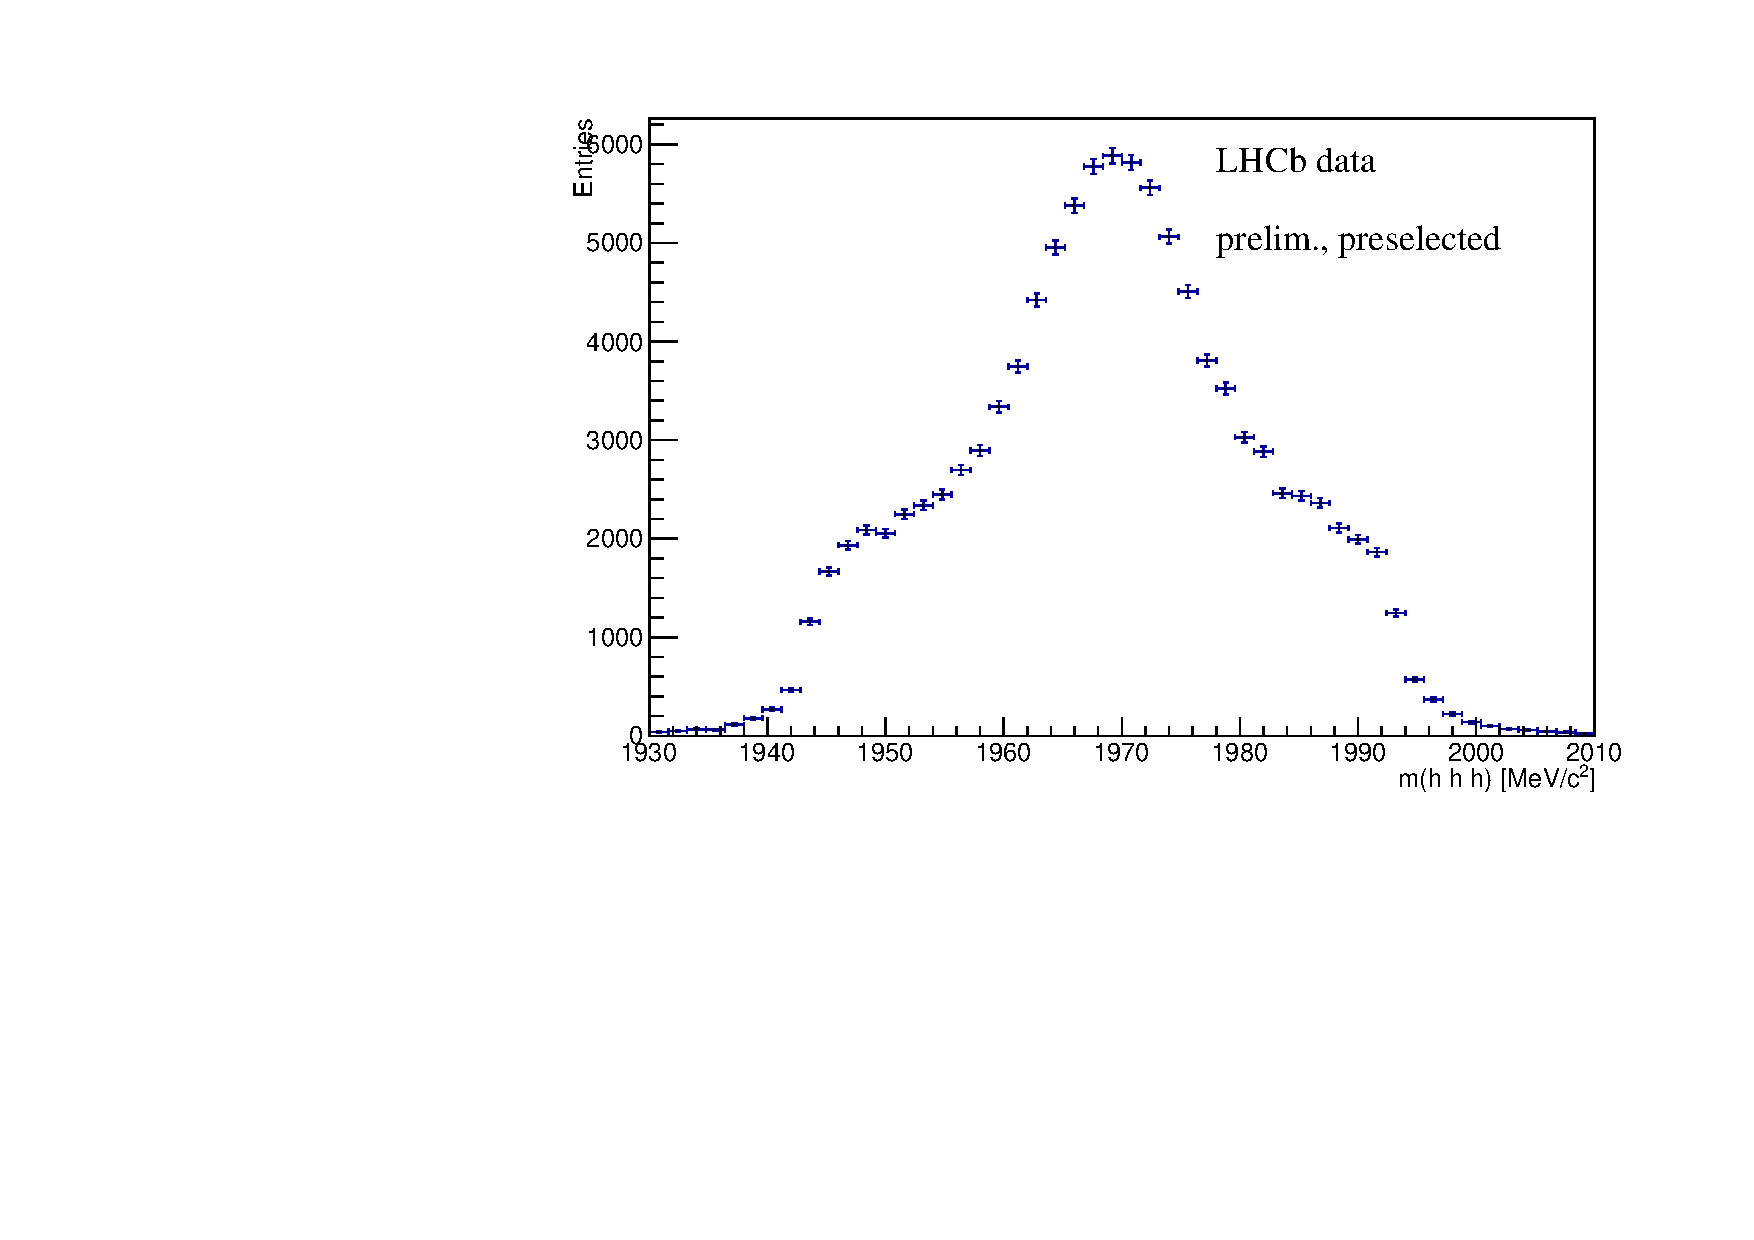
\includegraphics[height=7.0cm,width=0.49\textwidth]{figs/Ds_MM_afterpresel.pdf}
%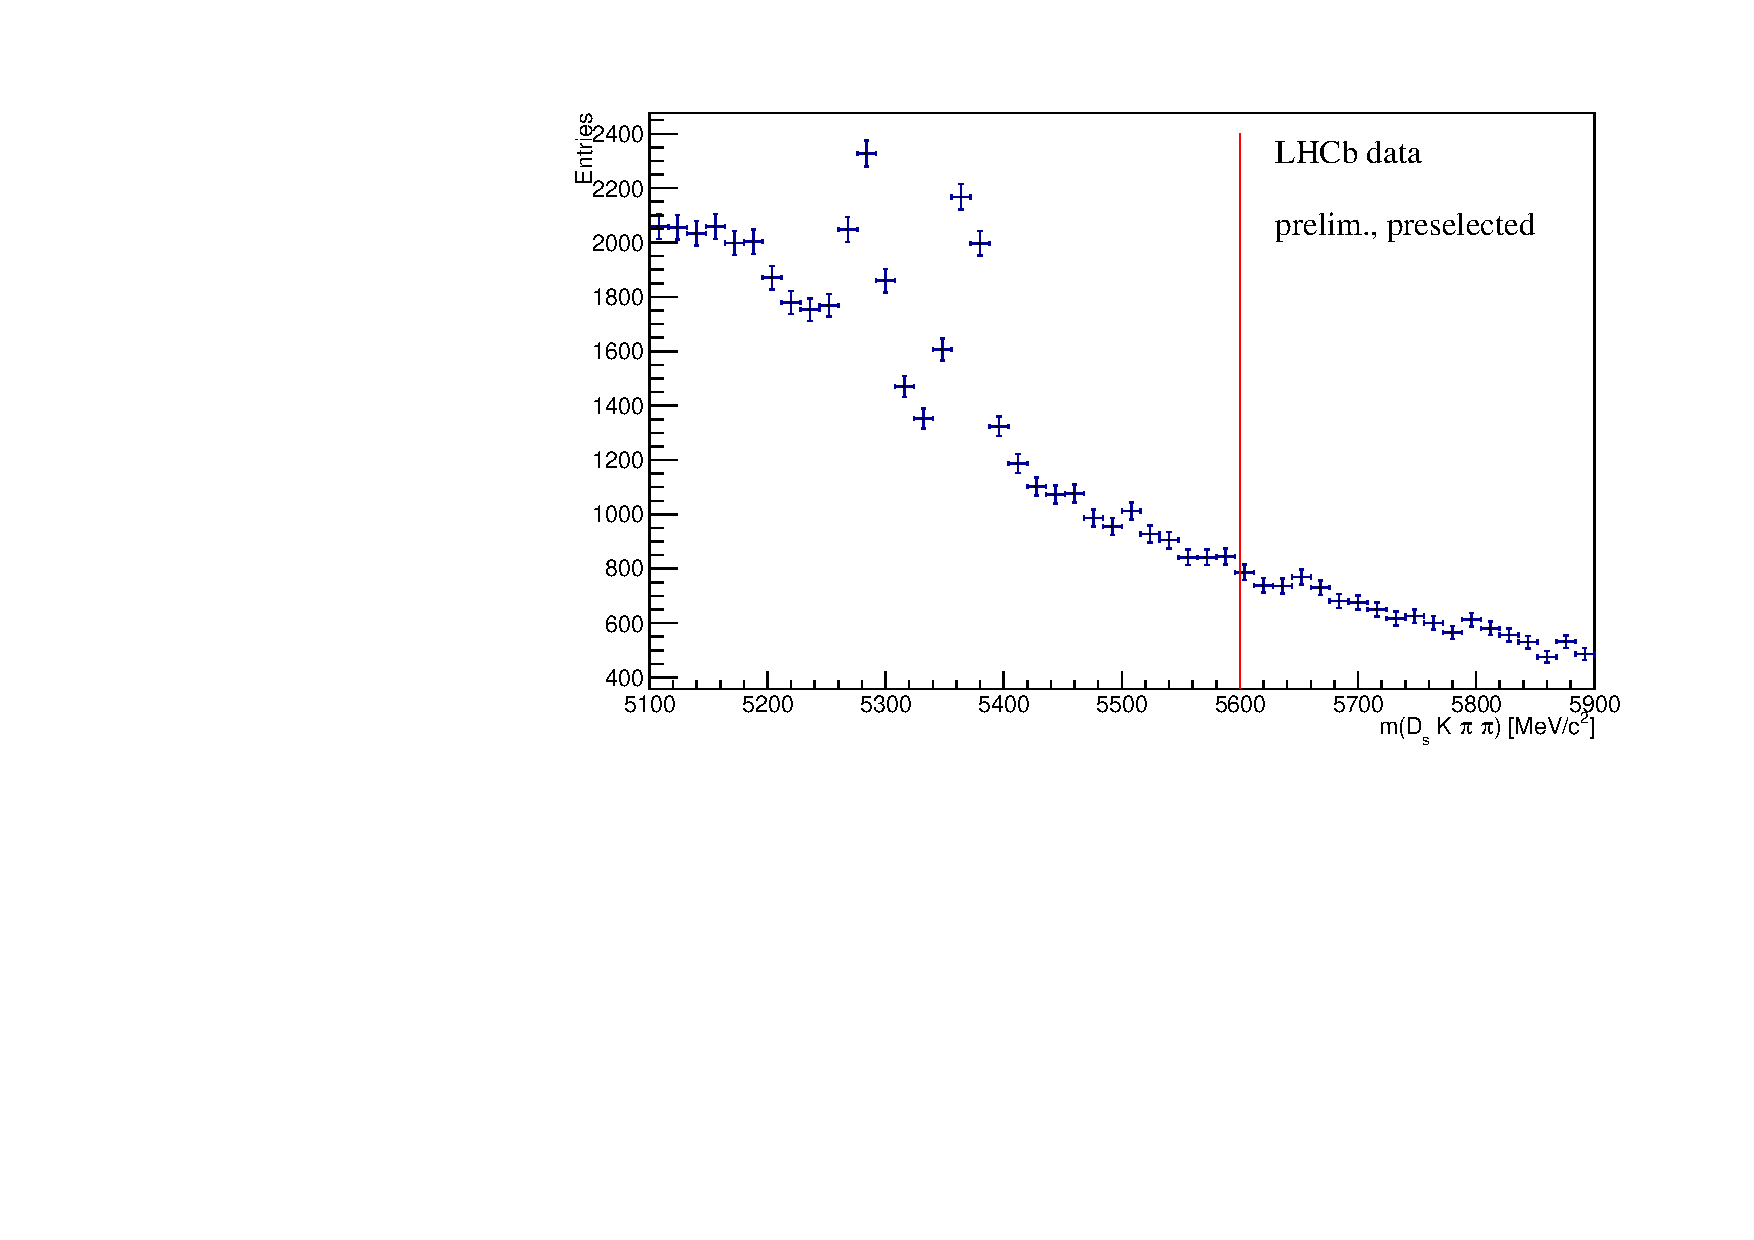
\includegraphics[height=7.0cm,width=0.49\textwidth]{figs/Bs_MM_afterpresel.pdf}
%%\vspace*{-0.2cm}
%\caption{Invariant mass distribution of preselected (left) $\Ds\to\hadron\hadron\hadron$ and (right) $\Bs\to\Ds\kaon\pion\pion$ candidates. 
%For the  $\Bs\to\Ds\kaon\pion\pion$ candidates, the region right from the red colored line with $m_{\Bs candidate}$ $>$ 5600 $\mevcc$ is used as background input for the boosted decision tree.}
%\label{fig:massforBDT}
%\end{figure}

%\newpage

\begin{figure}[h]
\centering
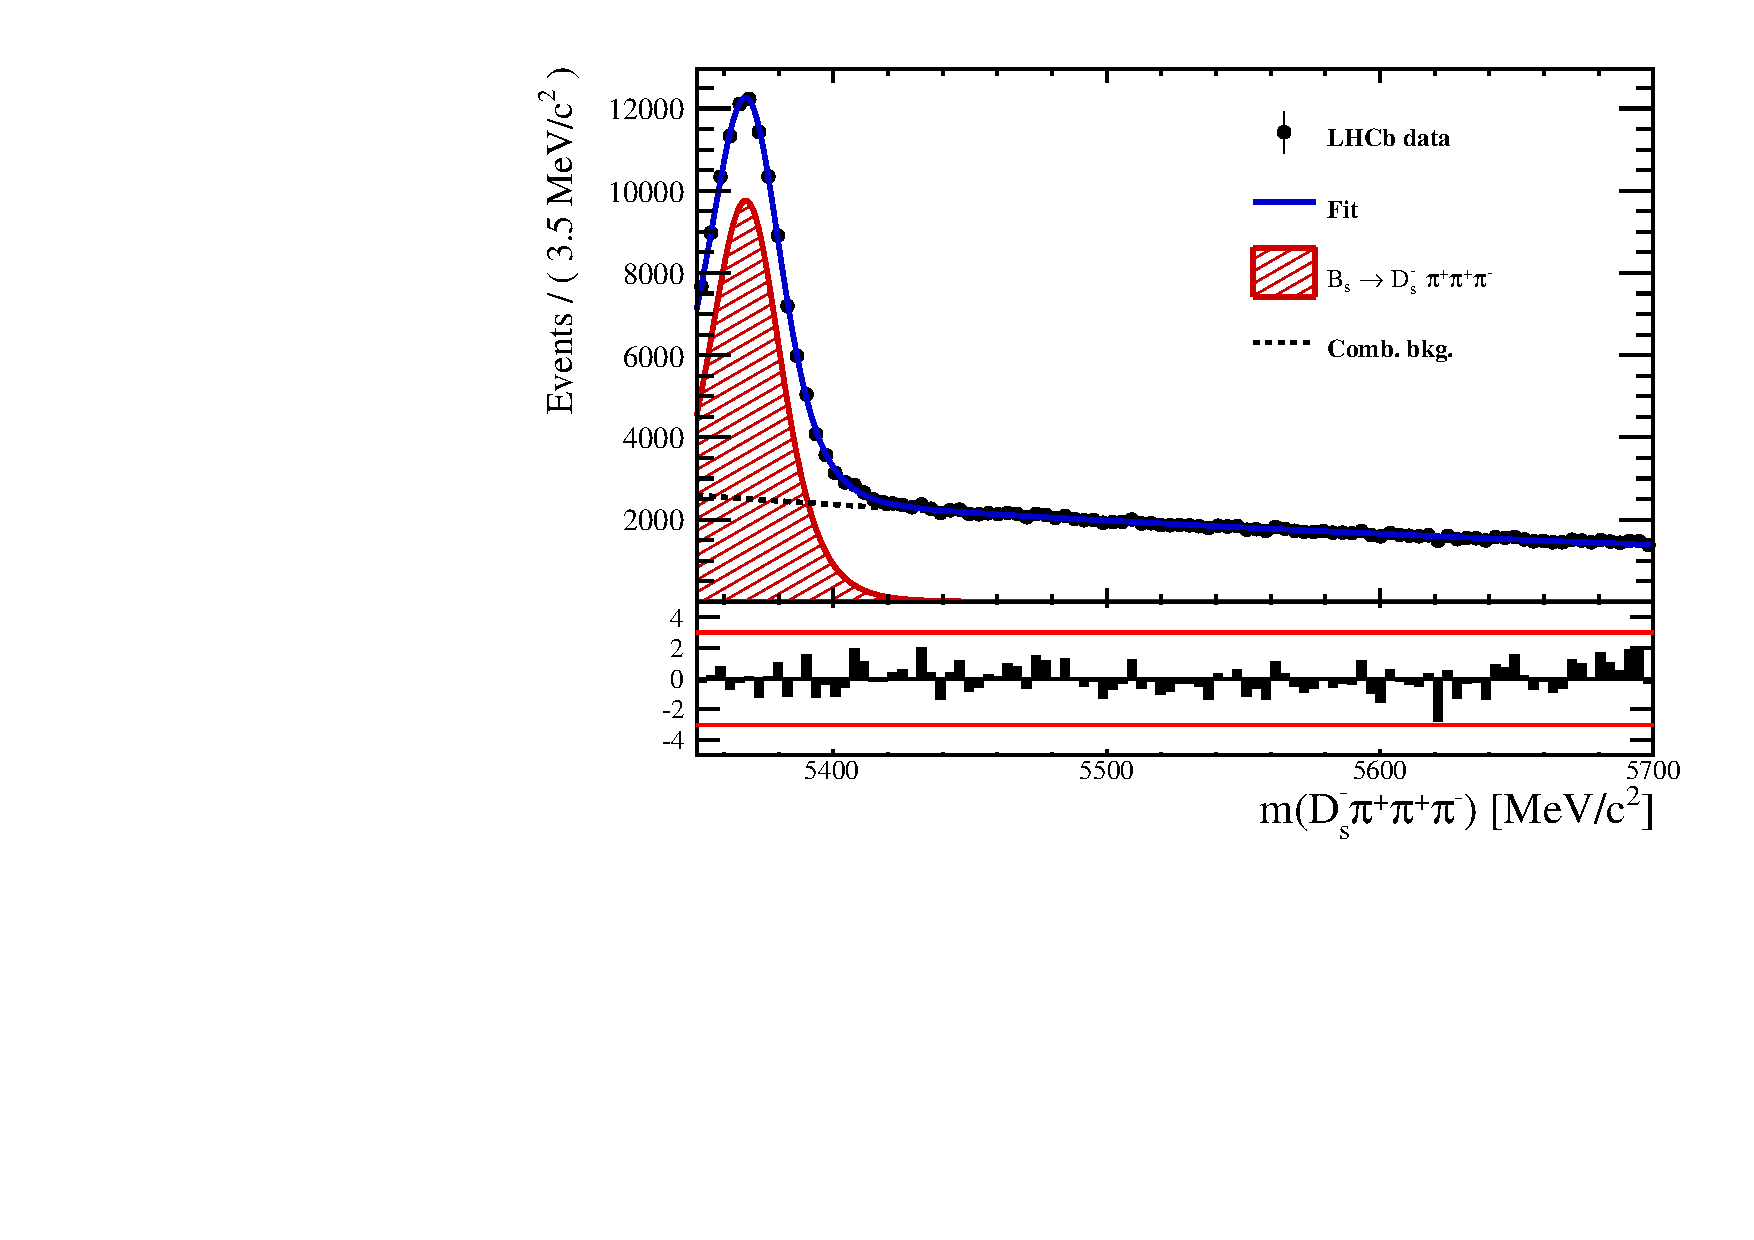
\includegraphics[height=!,width=0.45\textwidth]{figs/MassFit/norm_preselected_pull.pdf}
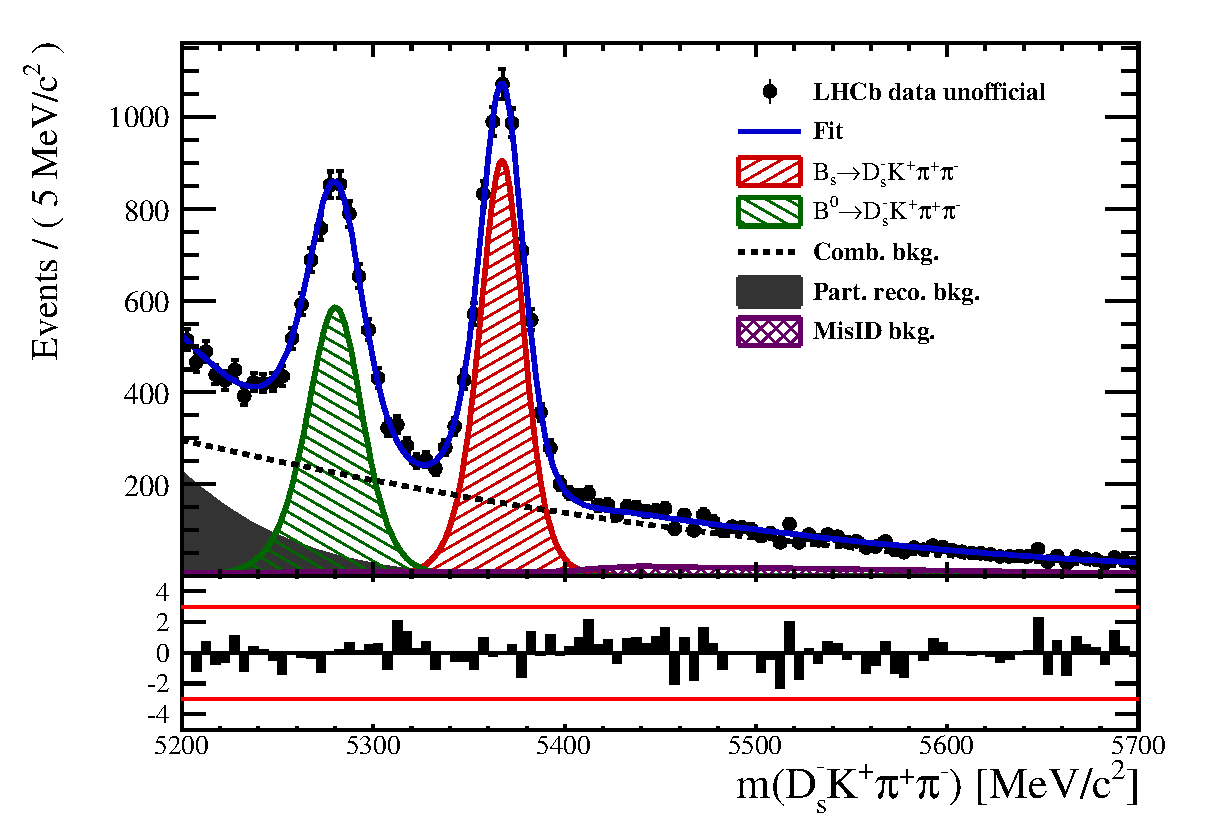
\includegraphics[height=!,width=0.45\textwidth]{figs/MassFit/signal_pull_00.eps}
\caption{Left: Reconstructed $B_s$ mass for $B_s\to D_s\pi\pi\pi$ events that pass the preselection (all categories combined). The fitted
PDF is shown in blue, the signal component in red and the background component in black.
\\Right: Reconstructed $B_s$ mass for $B_s\to D_sK\pi\pi$ events that pass the $BDTG > 0$ requirement (all categories combined). }
\label{fig:massFit_preselected}
\end{figure}
\begin{figure}[h]
\centering
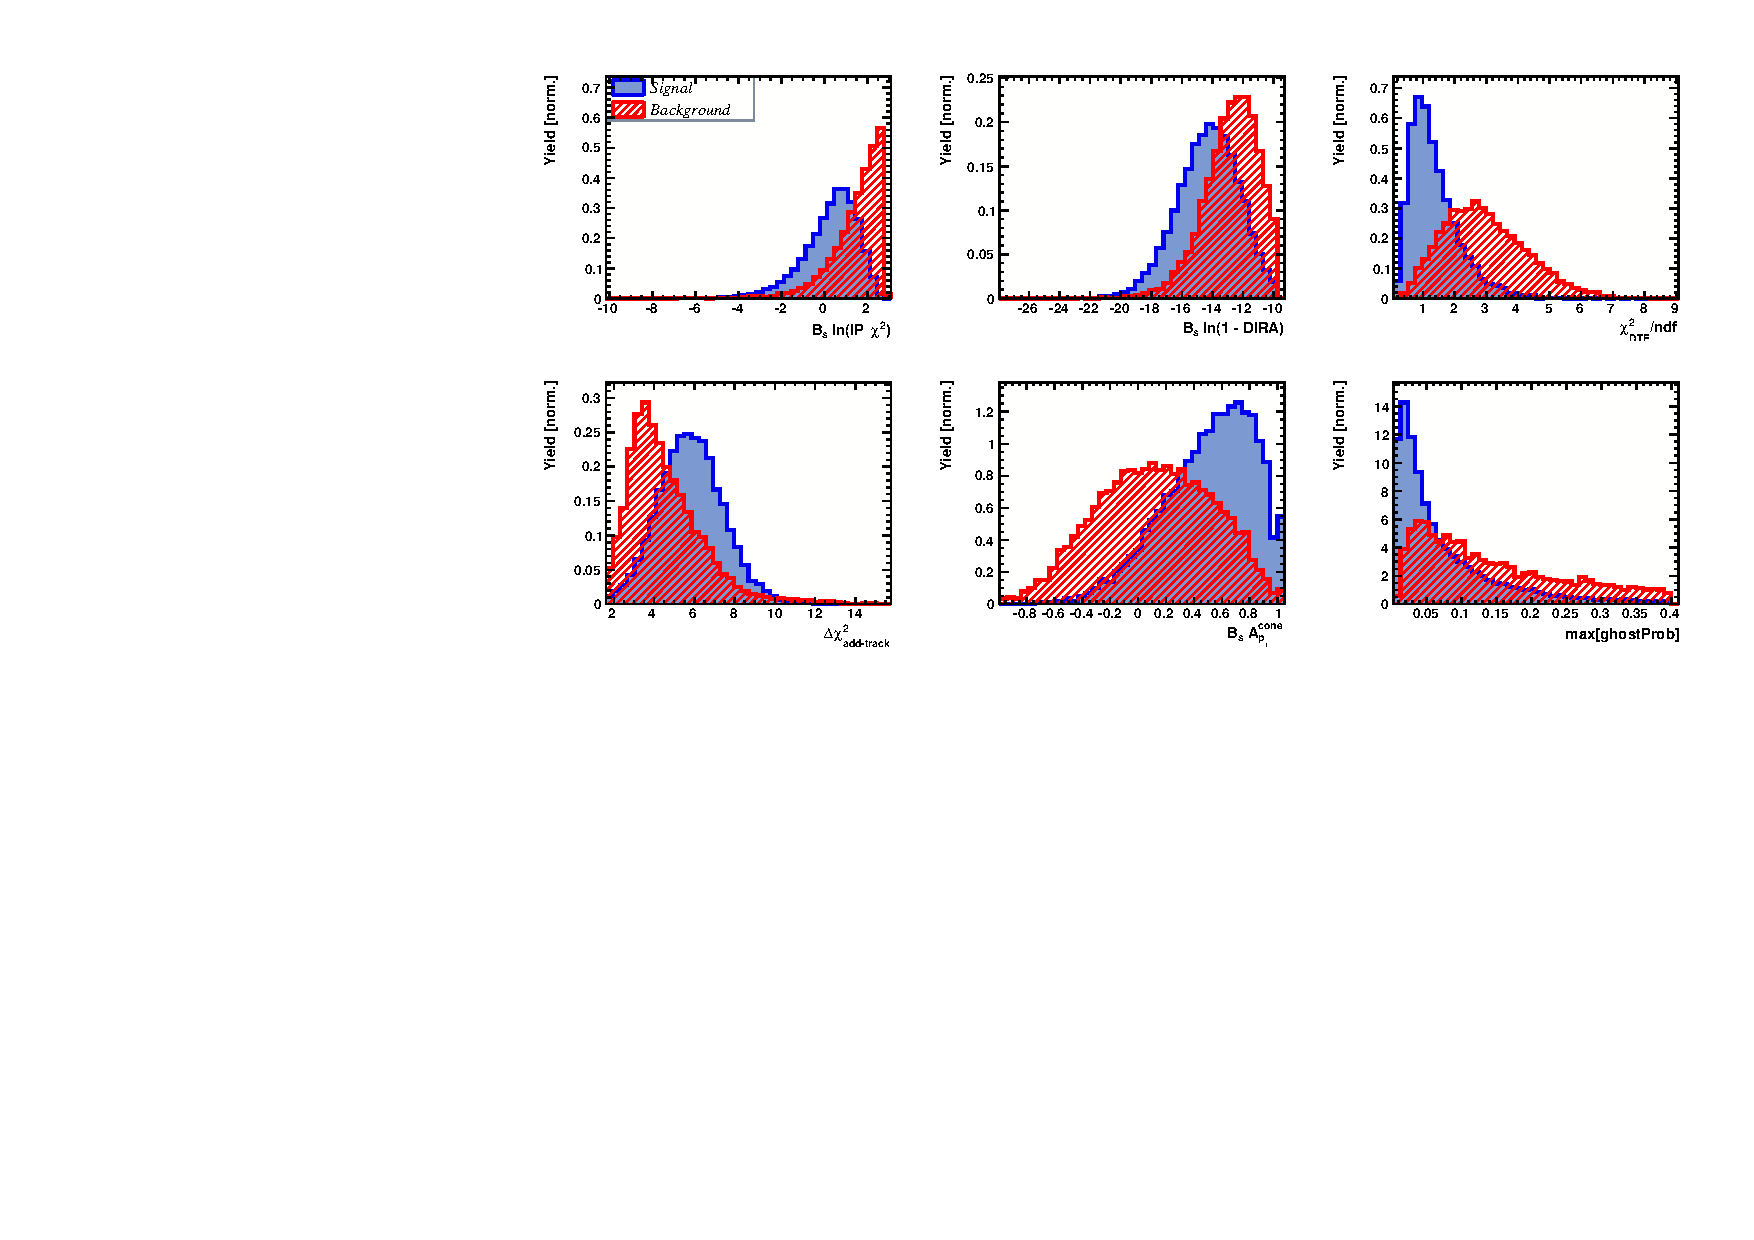
\includegraphics[height=!,width=0.8\textwidth]{figs/TMVA/BDTG_Data_all_all_all/variables_id_c1.pdf}
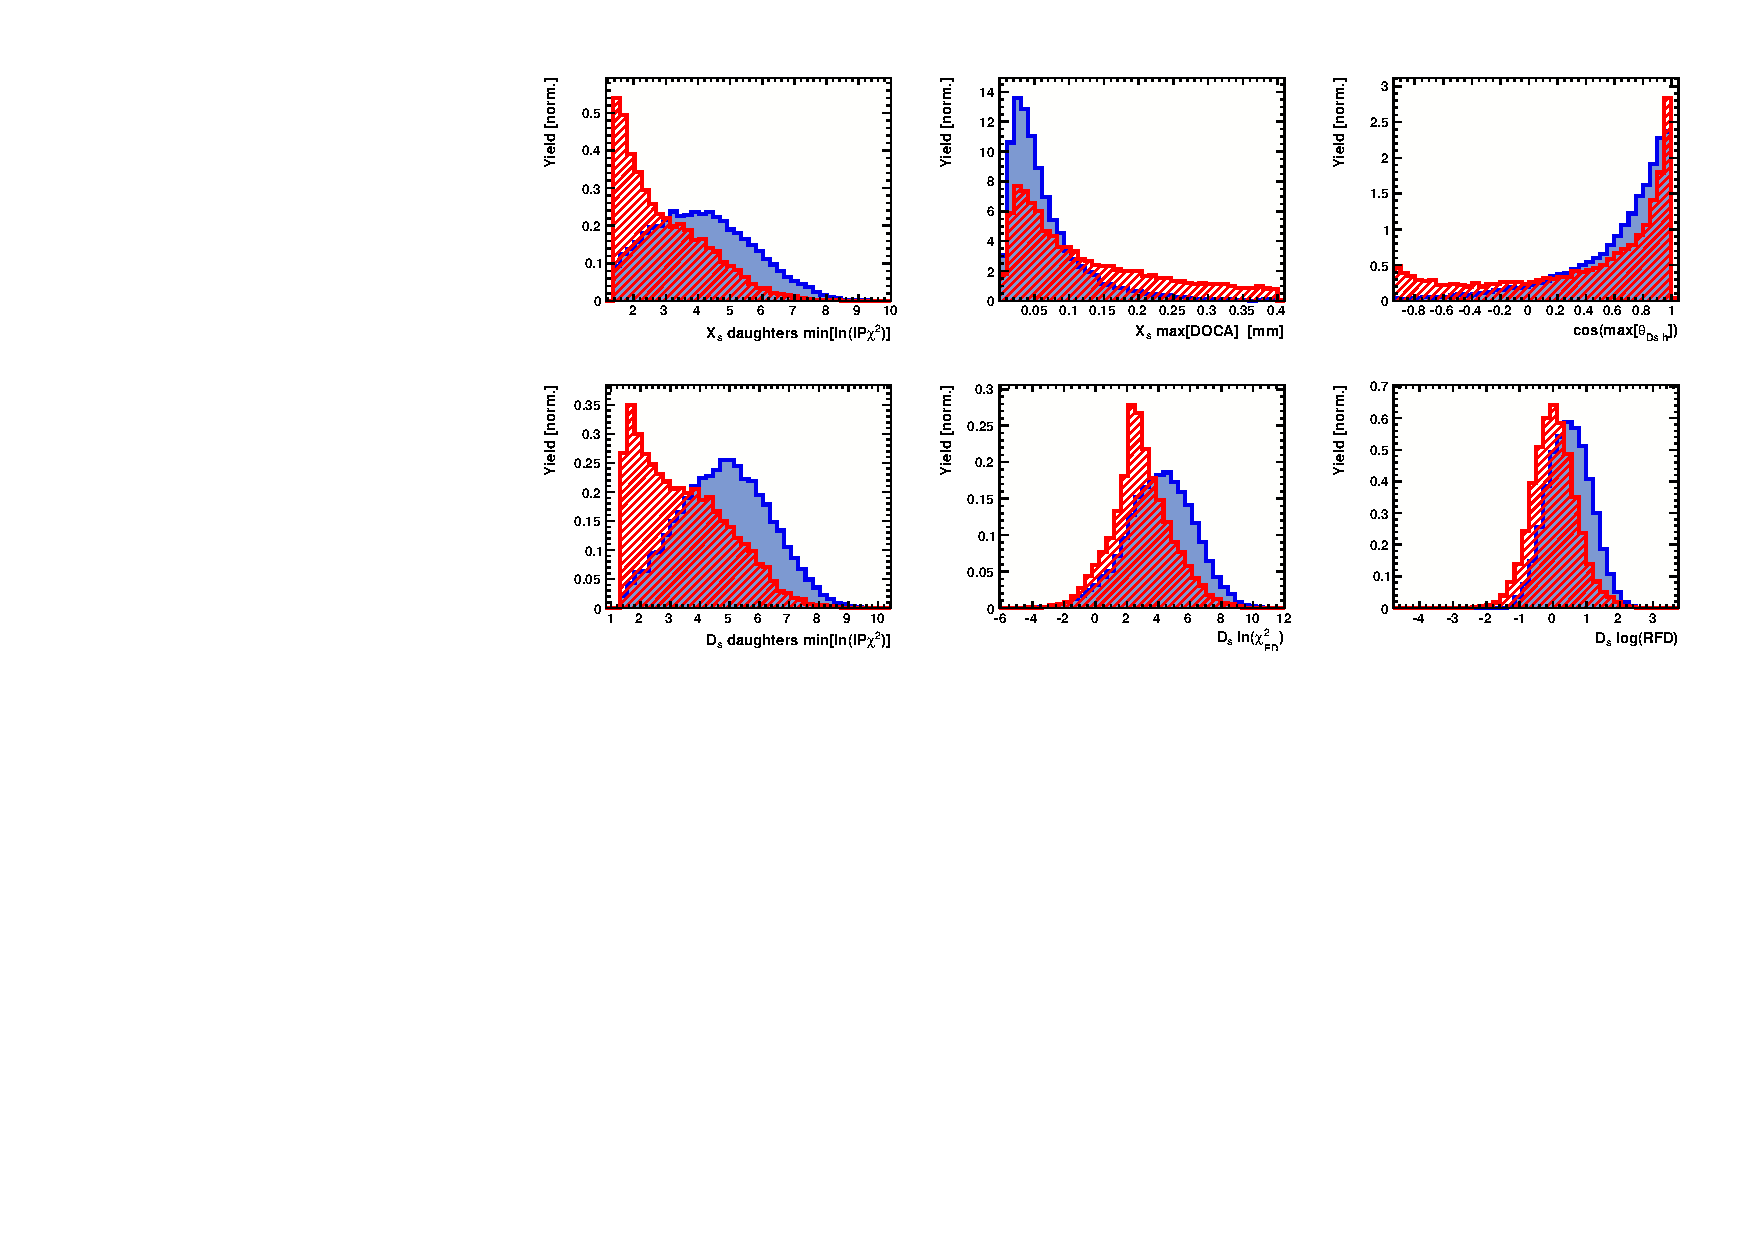
\includegraphics[height=!,width=0.8\textwidth]{figs/TMVA/BDTG_Data_all_all_all/variables_id_c2.pdf}
\caption{Discriminating variables used to train the BDTG for all data categories combined.}
\label{fig:varsBDT}
\end{figure}

\begin{figure}[h]
\centering
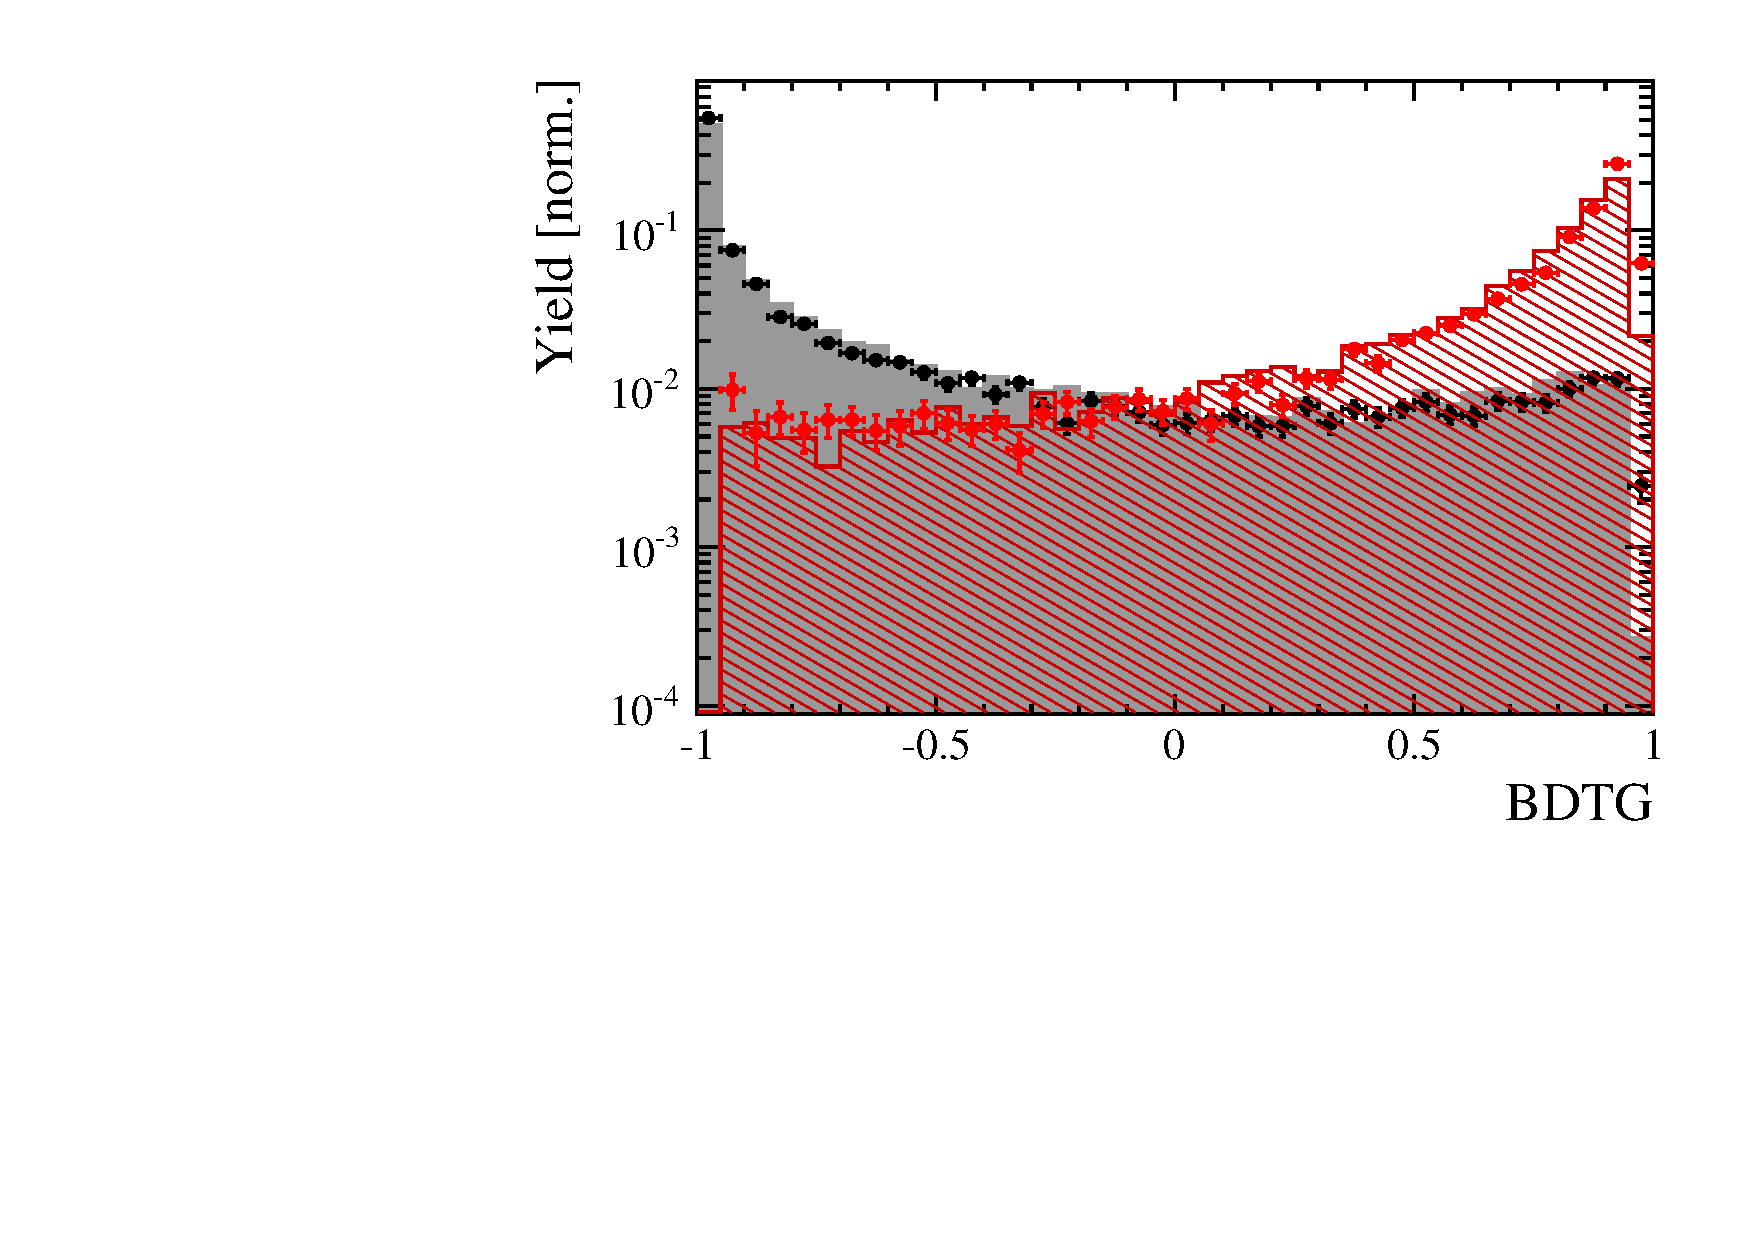
\includegraphics[height=!,width=0.4\textwidth]{figs/TMVA/BDTG_Run1.pdf}
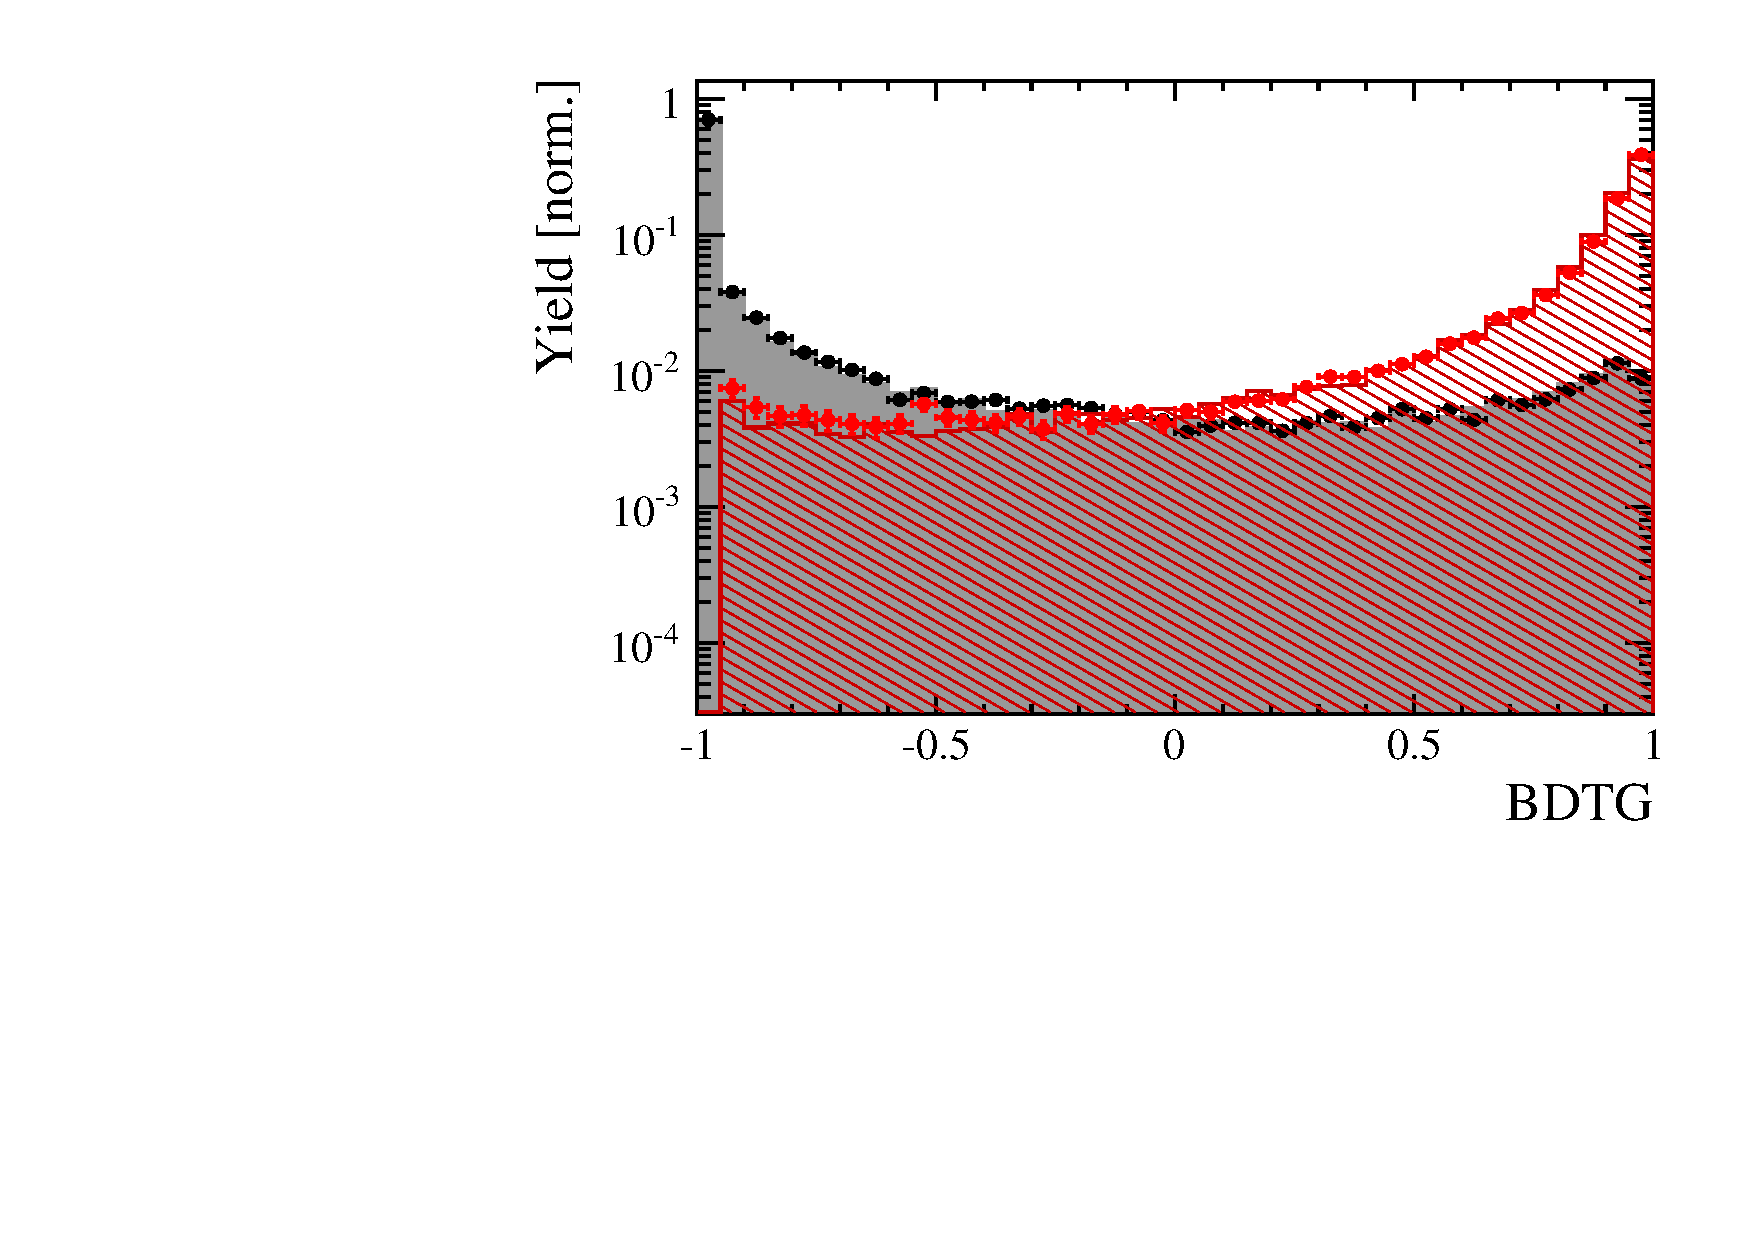
\includegraphics[height=!,width=0.4\textwidth]{figs/TMVA/BDTG_Run2.pdf}
\caption{Signal (red) and background (black) distributions for the BDTG response for Run-I (left) and Run-II (right) data. 
Filled histograms (data points) show the BDTG response for the \textsf{L0-TOS} (\textsf{L0-TIS}) category.
Even and odd test samples are combined.
}
\label{fig:BDTG}
\end{figure}

\subsubsection{Final selection}

The cut on the BDTG output is optimized using the signal significance as figure of merit:
\begin{equation}
	\text{FOM}(\text{BDTG}) = \frac{N_s(\text{BDTG})}{\sqrt{N_s (\text{BDTG})+ N_b(\text{BDTG})}}
\end{equation}
where $N_{s}(\text{BDTG})$ is the $B_s \to D_s K \pi \pi$ signal yield for a given BDTG cut and $N_{b}(\text{BDTG})$ is the combinatorial background yield in the signal region ($m(D_sK\pi\pi) = m_{B_s} \pm 40 \mev$).
To compute the yields as function of the BDTG cut, we use the BDTG efficiencies, $\epsilon_{s,b}$, evaluated on the corresponding test samples.
To fix the overall scale, it is required to know the yields at (at least) one point of the scanned range.
We arbitrarily choose this fix point to be BDTG $> 0$ and perform a fit to the reconstructed $B_s$ mass as described in Sec.~\ref{sec:massFits} to obtain the yields $N_{s,b}(0)$,
see Fig.~\ref{fig:massFit_preselected}(right).
These yields are then efficiency corrected to calculate the yields for a given BDTG cut: 
\begin{equation}
N_{s,b}(\text{BDTG}) = N_{s,b}(0) \cdot \frac{\epsilon_{s,b}(\text{BDTG})}{\epsilon_{s,b}(0)}.
\end{equation}
Figure \ref{fig:scanBDT} shows the resulting BDTG scans for each training category.
\begin{figure}[h]
\centering
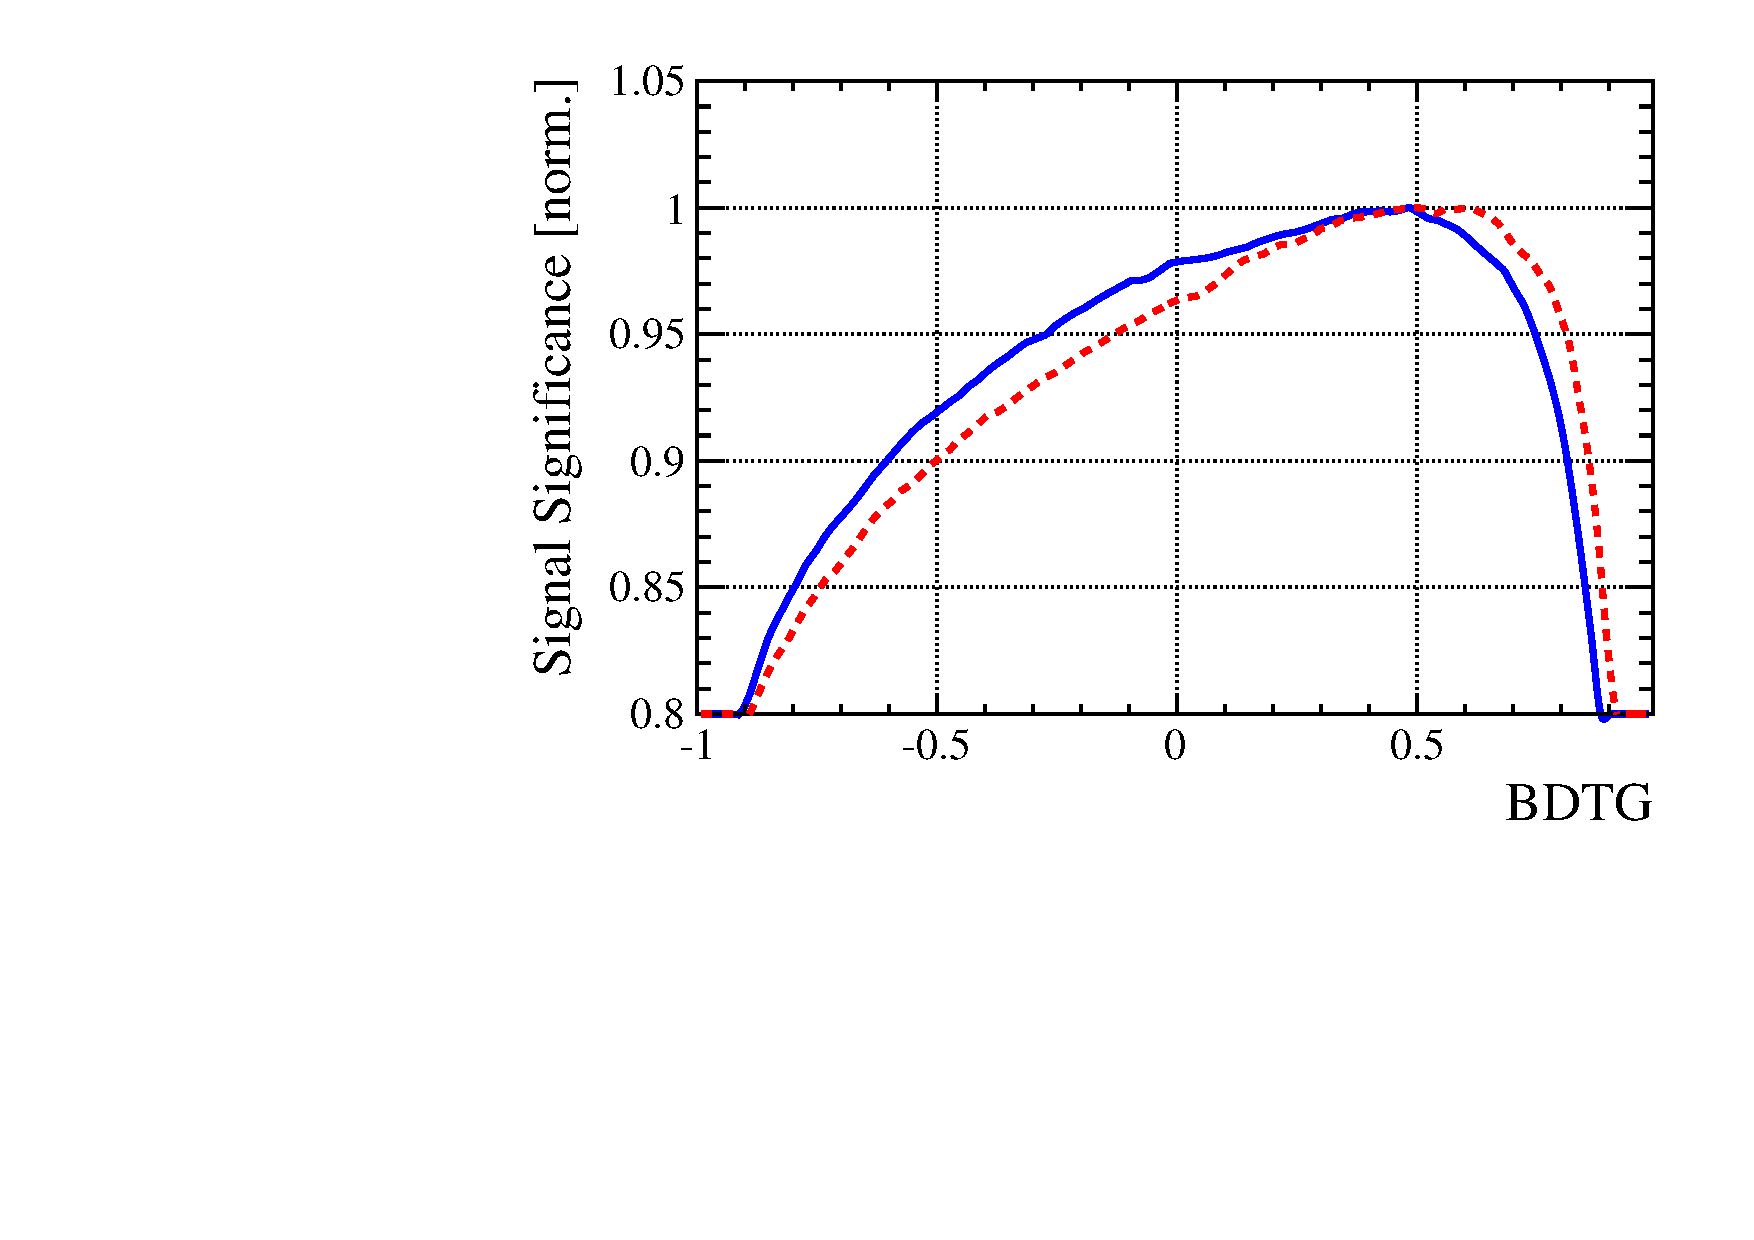
\includegraphics[height=!,width=0.4\textwidth]{figs/TMVA/BDT_scan_Run1.pdf}
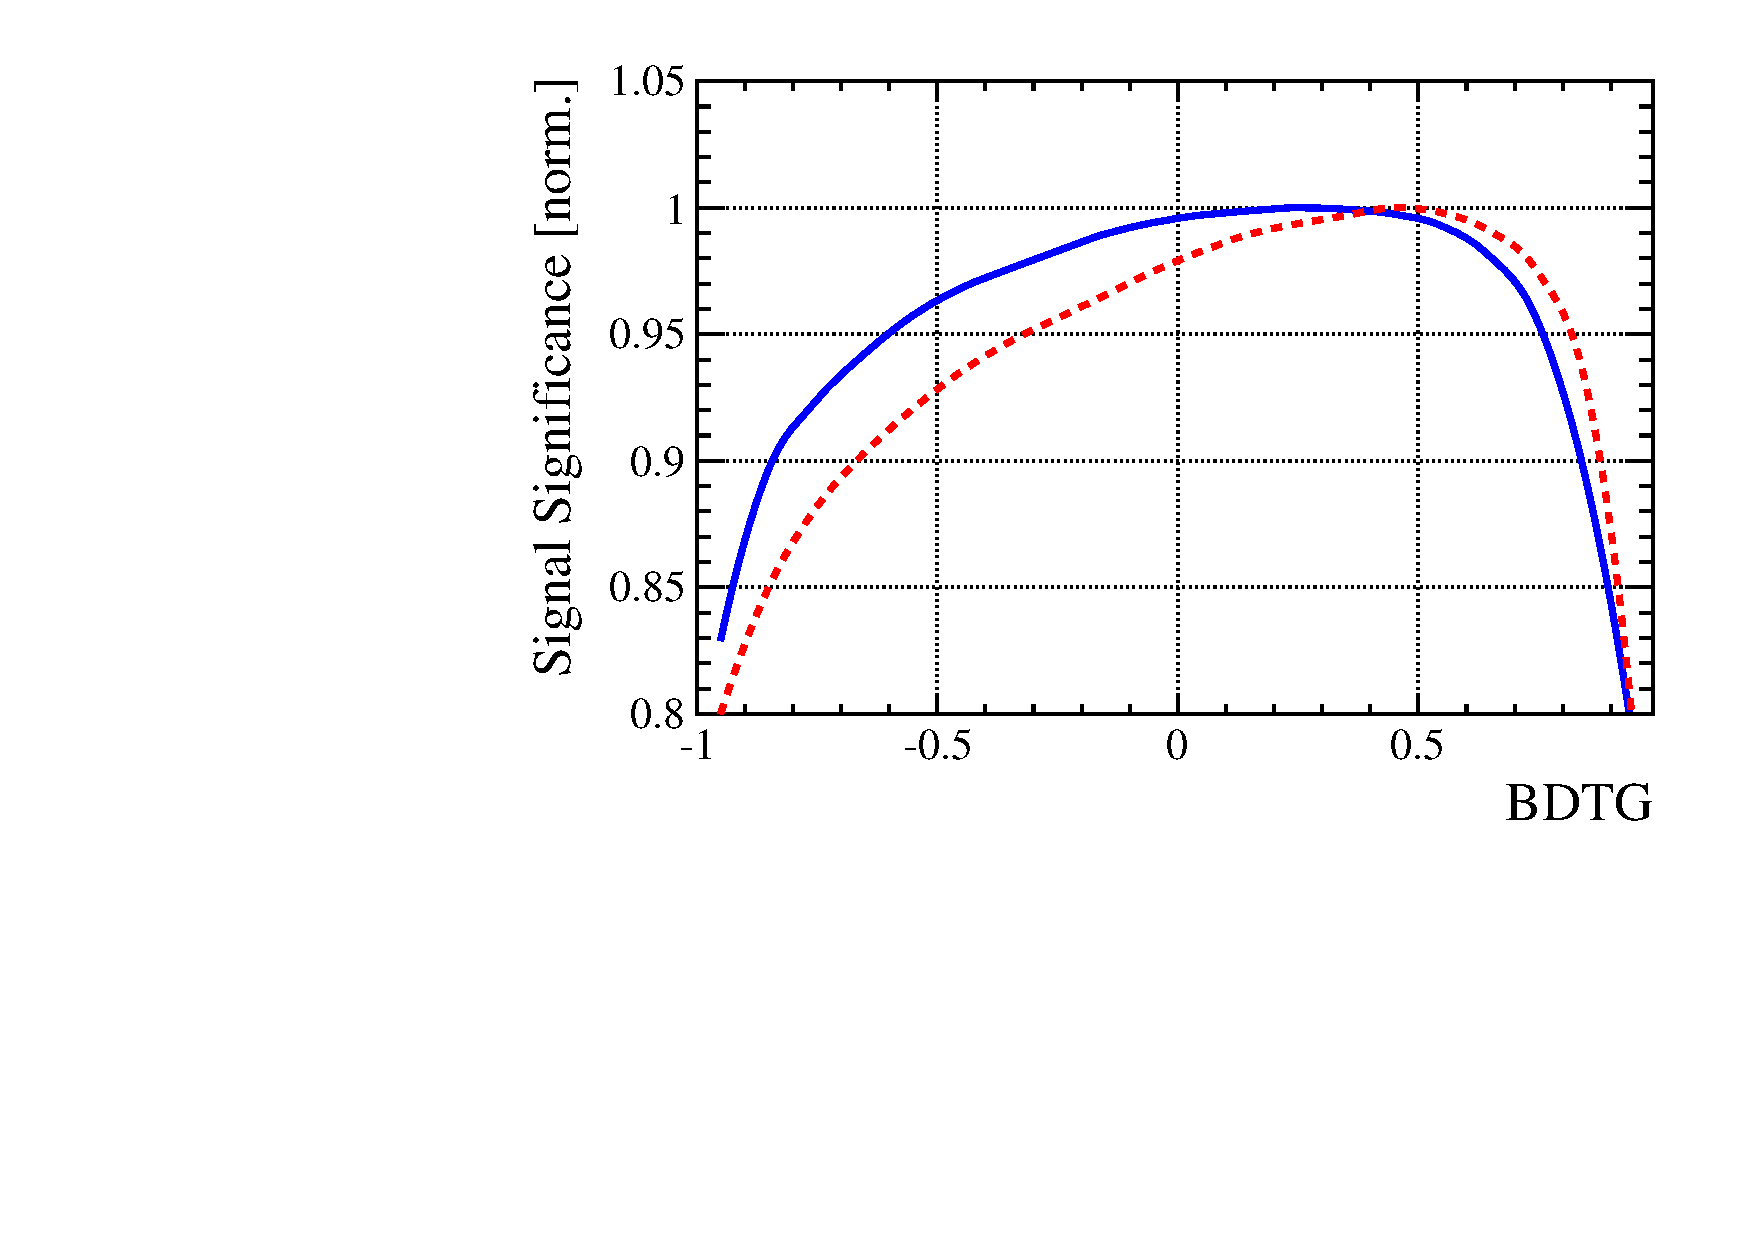
\includegraphics[height=!,width=0.4\textwidth]{figs/TMVA/BDT_scan_Run2.pdf}
\caption{Signal significance as function of the applied cut on the BDTG response for Run-I (left) and Run-II (right) data.
The scans for the \textsf{L0-TOS} (\textsf{L0-TIS}) category are shown in blue (red).
The signal significance is normalized to be 1 at the optimal BDTG cut value.
}
\label{fig:scanBDT}
\end{figure}


%The relative importance of the input variables for the BDTG training is summarized in Table \ref{table:InputVars}.
%
%\begin{table}[h]
%\centering
% \begin{tabular}{l c}
%Variable & relative importance [$\%$]\\
%  \hline
%pi\_minus\_ptasy\_1.00 & 7.32\\
%log\_Ds\_FDCHI2\_ORIVX & 7.23\\
%K\_plus\_ptasy\_1.00 & 7.17\\
%log\_Ds\_DIRA & 6.96\\
%Bs\_ENDVERTEX\_CHI2 & 6.82\\
%max\_ghostProb & 6.76\\
%pi\_plus\_ptasy\_1.00 & 6.57\\
%log\_DsDaughters\_min\_IPCHI2 & 6.21\\
%log\_Bs\_DIRA & 6.15\\
%K\_plus\_fromDs\_ptasy\_1.00 & 6.10\\
%log\_XsDaughters\_min\_IPCHI2 & 5.87\\
%K\_minus\_fromDs\_ptasy\_1.00 & 5.62\\
%cos(Ds h) & 5.58\\
%log\_Bs\_IPCHI2\_OWNPV & 5.08\\
%log\_Bs\_FDCHI2\_OWNPV & 4.04\\
%Xs\_max\_DOCA & 3.98\\
%pi\_minus\_fromDs\_ptasy\_1.00 & 2.59\\
%\end{tabular}
%\caption{Summary of the relative importance of each variable in the training of the BDTG.}
%\label{table:InputVars}
%\end{table}


\clearpage

\begin{table}[h]
\centering
\caption{Offline selection requirements for $D_s \to 3 h$ candidates.}
\resizebox{\linewidth}{!}{
 \renewcommand{\arraystretch}{1.}
 \small
 \begin{tabular}{l l l}
\hline
\hline
 & Description & Requirement  \\
\hline
$D_s \to h h h$ &  $m(hhh)$ & = $m_{D_s} \pm 25 \mev$  \\
%& $p_T $ & $> 1600 \mev$\\
\\
$D_s^- \to K K \pi^-$  & $D^0$ veto  & $m(K K) < 1840$ MeV \\
\\
$D_s^- \to \phi \pi^-$ & $m(KK)$  & $= m_{\phi} \pm 12$ MeV \\
& PIDK($K^+$) & $> -10$ \\
& PIDK($K^-$) & $> -10$ \\
& PIDK($\pi^-$) & $< 20$ \\
&  $\chi^{2}_{FD}$ & $> 0$ \\
&  FD in $z$  &$ > -1$ \\
& $D^-$ veto  & $m(\Kp K^-_\pi \pim) \ne m(D^-) \pm 40$ MeV  $||$ $\text{PIDK}(K^-) > 5$\\
& $\Lambda_c$ veto  & $m(\Kp K^-_p \pim) \ne m(\Lambda_c) \pm 40$ MeV   $||$ $\text{PIDK}(K^-)-\text{PIDp}(K^-) > 2$ \\
\\
$D_s^- \to K^{*}(892) K^-$ & $m(KK)$  & $\ne m_{\phi} \pm 12$ MeV \\
& $m(K^+\pi^-)$  & $= m_{K^{*}(892)} \pm 75$ MeV \\
& PIDK($K^+$) & $> -10$ \\
& PIDK($K^-$) & $> 0$ \\
& PIDK($\pi^-$) & $< 10$ \\
&  $\chi^{2}_{FD}$ & $> 0$ \\
&  FD in $z$  &$ > 0$ \\
& $D^-$ veto  & $m(\Kp K^-_\pi \pim) \ne m(D^-) \pm 40$ MeV  $||$ $\text{PIDK}(K^-) > 15$\\
& $\Lambda_c$ veto  & $m(\Kp K^-_p \pim) \ne m(\Lambda_c) \pm 40$ MeV   $||$ $\text{PIDK}(K^-)-\text{PIDp}(K^-) > 5$ \\
\\
$D_s^- \to (K K \pi^-)_{NR}$ & $m(KK)$  & $\ne m_{\phi} \pm 12$ MeV \\
& $m(K^+\pi^-)$  & $\ne m_{K^{*}(892)} \pm 75$ MeV \\
& PIDK($K^+$) & $> 5$ \\
& PIDK($K^-$) & $> 5$ \\
& PIDK($\pi^-$) & $< 10$ \\
&  $\chi^{2}_{FD}$ & $> 4$ \\
&  FD in $z$  &$ > 0$ \\
& $D^-$ veto  & $m(\Kp K^-_\pi \pim) \ne m(D^-) \pm 40$ MeV  $||$ $\text{PIDK}(K^-) > 15$\\
& $\Lambda_c$ veto  & $m(\Kp K^-_p \pim) \ne m(\Lambda_c) \pm 40$ MeV  $||$ $\text{PIDK}(K^-)-\text{PIDp}(K^-) > 5$ \\
\\
$D_s^- \to \pi \pi \pi$ & PIDK($\pi$) & $< 10$  \\
& PIDp($\pi$) & $< 20$ \\
& $D^0$ veto  & $m(\pip \pim) < 1700$ MeV\\
&  $\chi^{2}_{FD}$ & $> 9$ \\
&  FD in $z$  &$ > 0$ \\
\\
$D_s^- \to K^- \pip \pim$ & PIDK($K$) & $> 8$  \\
& PIDK($\pi$) & $< 5$ \\
& PIDp($\pi$) & $< 20$ \\
& $D^0$ veto  & $m(K^- \pip) < 1750$ MeV \\
&  $\chi^{2}_{FD}$ & $> 9$ \\
&  FD in $z$  &$ > 0$ \\
& $D^-$ veto  & $m(K^-_\pi \pip \pim) \ne m(D^-) \pm 40$ MeV  $||$ $\text{PIDK}(K^-) > 15$\\
& $\Lambda_c$ veto  & $m(K^-_p \pip \pim) \ne m(\Lambda_c) \pm 40$ MeV  $||$ $\text{PIDK}(K^-)-\text{PIDp}(K^-) > 5$ \\
\\
\hline
\hline
\end{tabular}
}
\label{table:selDs}
\end{table}


\begin{table}[h]
\centering
\caption{Offline selection requirements for $B_s\to D_s K \pi\pi (D_s \pi\pi\pi)$ candidates.}
%\resizebox{\linewidth}{!}{
 \renewcommand{\arraystretch}{1.}
 \small
 \begin{tabular}{l l l}
\hline
\hline
 & Description & Requirement  \\
\hline
$B_s \to D_s h \pi \pi$  & $m(D_s h \pi \pi)$ & $> 5200 \mev$ \\
&  $\chi^{2}_{vtx}/\text{ndof}  $&$ <  8$ \\
& DIRA &$ > 0.99994$ \\
& $\chi^{2}_{FD}$ & $> 100$ \\
& $\chi^{2}_{IP}$ & $< 16$ \\
&  $\chi^{2}_{DTF}/\text{ndof} $&$   <  15 $ \\
&  $\Delta\chi^{2}_{add-track} $&$   >  2 $ \\
& $\cos(\text{max} \, \theta_{\Ds h_{i}})$ &$   > -0.9 $ \\
& $t$  & $ > 0.4 \ps$ \\
& $\delta t$  & $ < 0.15 \ps$ \\
& Phasespace region & $m(h\pi\pi) < 1.95 \gev$ \\ & & $m(h\pi) < 1.2 \gev$ \\ & & $m(\pi\pi) < 1.2 \gev$ \\
& Wrong PV veto & nPV = 1 $||$  $\text{min}(\Delta\chi^{2}_{IP}) > 20$ \\
& BDTG &  $> 0.35$ [Run-I,\textsf{L0-TOS}] \\
& & $> 0.45$ [Run-I,\textsf{L0-TIS}] \\
& & $> 0.25$ [Run-II,\textsf{L0-TOS}] \\
& & $> 0.45$ [Run-II,\textsf{L0-TIS}] \\
\\
$X_s^+ \to K^+ \pi^+ \pi^-$  & PIDK(K) & $> 10$ \\
& PIDK($\pi^+$) & $< 10$ \\
& PIDK($\pi^-$) & $< 0$ \\
& $D_s$ veto & $m(\Kp \pip \pi^-_K) \ne m(D_s) \pm 20$ MeV $||$ PIDK($\pim$) $< -5$ \\
%& Semi.-lep. veto & isMuon($K^+$) = 0 \\
\\
$X_d^+ \to \pi^+ \pi^+ \pi^-$  & PIDK($\pi^+$) & $< 0$ \\
& PIDK($\pi^-$) & $< 10$ \\
& $D_s$ veto & $m(\pip \pi^+_K \pim) \ne m(D_s) \pm 20$ MeV $||$ PIDK($\pip$) $< -5$ \\
%& Semi.-lep. veto & isMuon($\pip$) = 0 \\
\\
All tracks & hasRich & $= 1$ \\
%& $p$ & $> 2500 \mev$ \\ 

\hline
\hline
\end{tabular}
%}
\label{table:selBs}
\end{table}


\clearpage
\subsection{Simulation}
\label{sec:Sim}

Several Monte Carlo (MC) samples are used in the analysis for acceptance and
background studies.
A full list of them is given in Tab.~\ref{table:mcSamples}.
In each case, the decay model includes a mixture of non-interfering resonances contributing to the bachelor system and a non-resonant (phase-space) component.
For $B_s \to D_s X_s$ these are:
25\% $X_s \to \pi ( K_1(1270) \to K \rho(770) )$, 
70\% $X_s \to \pi ( K_1(1400) \to K^*(892) \pi)$
and 5\% $X_s \to K \pi \pi$ (non-resonant).
And similar for $B_s \to D_s X_d$:
85\% $X_d \to \pi ( a_1(1260) \to \rho(770) \pi )$, 
10\% $X_d \to \pi ( a_1(1260) \to \sigma \pi)$
and 5\% $X_d \to K \pi \pi$ (non-resonant).
All MC samples are generated using \textsf{Pythia8}, reconstructed using
\textsf{Reco14c}, \textsf{Reco15} and \textsf{Reco16} for Run-I, 15 and 16 data and
selected using the same criteria as in data.
%\newline
%\\
%\pretextcomment{
%All samples indicated with 'Requested' have been requested in Dec. 17 and are expected to be available soon.
%}

\begin{table}[h]
\centering
\caption{List of simulated samples used in the analysis.}
\resizebox{\linewidth}{!}{
 \renewcommand{\arraystretch}{1.2}
% \small
 \begin{tabular}{l l l l l l l ll}
\hline
\hline
Decay & Event Type &  \multicolumn{1}{c}{\textsf{Sim}} &  \multicolumn{4}{c}{Statistics} & Filter \\
 &  &  & 11 & 12 & 15 & 16 &  \\

\hline
$B_s \to (D_s \to K K \pi) K \pi\pi$  & 13266007   & 08i & 1.2 M & 1.2 M & - & -   & Generator Level  \\
$B_s \to (D_s \to K K \pi) K \pi\pi$  & 13266008  & 09c & 70 k & 80 k & 50 k & 100 k  & Generator Level, Stripping  \\
$B_s \to (D_s \to K \pi \pi) K \pi\pi$  & 13266058 & 09c  & 70 k & 80 k & 50 k & 100 k   & Generator Level, Stripping  \\
$B_s \to (D_s \to \pi \pi \pi) K \pi\pi$  & 13266038  & 09c &  70 k & 80 k & 50 k & 100 k  & Generator Level, Stripping  \\
\\
$B_s \to (D_s \to K K \pi) \pi \pi\pi$  & 13266006 & 08i   & 1.2 M & 1.2 M & - & -   & Generator Level  \\
$B_s \to (D_s \to K K \pi) \pi \pi\pi$  & 13266068  & 09c & 70 k & 80 k & 50 k & 100 k   & Generator Level, Stripping  \\
$B_s \to (D_s \to K \pi \pi) \pi \pi\pi$  & 13266088  & 09c & 70 k & 80 k & 50 k & 100 k   & Generator Level, Stripping  \\
$B_s \to (D_s \to \pi \pi \pi) \pi \pi\pi$  & 13266078 & 09c  &70 k & 80 k & 50 k & 100 k    & Generator Level, Stripping  \\
\\
$B_s \to D_s^* \pi \pi\pi, D_s \to KK \pi$  & 13266201 & 08i   & 1.2 M & 1.2 M & - & -    & Generator Level  \\


\hline
\hline
\end{tabular}
}
\label{table:mcSamples}
\end{table}

